% Five-Column Connect Four Is a Draw at Every Finite Height
% Single-file source. Build: pdflatex five_columns_draw_en.tex (run three times from a clean directory).
% Needs a standard TeX Live (mathpazo, booktabs, tabularx, cleveref, tikz, hyperref).
% ===== preamble.tex =====
\documentclass[11pt,a4paper]{article}

\usepackage[a4paper,margin=22mm]{geometry}
\usepackage[T1]{fontenc}
\usepackage{mathpazo}
\usepackage[scaled=0.90]{helvet}
\renewcommand{\ttdefault}{lmtt}
\usepackage{microtype}

\usepackage{amsmath,amssymb,amsthm,mathtools}
\usepackage{xcolor}
\usepackage{booktabs,tabularx,array}
\usepackage[font=small,labelfont=bf]{caption}
\usepackage{enumitem}
\usepackage{tikz}
\usetikzlibrary{arrows.meta,positioning,calc,decorations.pathreplacing}
\PassOptionsToPackage{obeyspaces,spaces}{url}
\usepackage{hyperref}
\usepackage[nameinlink,capitalise]{cleveref}

\definecolor{primary}{RGB}{20,54,93}
\definecolor{accent}{RGB}{18,110,98}
\definecolor{warn}{RGB}{168,50,50}
\definecolor{gold}{RGB}{176,120,20}
\definecolor{softbg}{RGB}{244,247,251}
\definecolor{gridgray}{RGB}{176,184,194}
\definecolor{stoneB}{RGB}{30,30,30}

\hypersetup{
  colorlinks=true,
  linkcolor=primary,
  citecolor=accent,
  urlcolor=primary,
  pdftitle={Five-Column Connect Four Is a Draw at Every Finite Height},
  pdfauthor={GPT, Claude, and Gemini}
}

\setlength{\parskip}{4pt plus 1pt minus 1pt}
\setlength{\parindent}{0pt}
\setlength{\emergencystretch}{3em}
\renewcommand{\arraystretch}{1.18}
\setlist{itemsep=2pt,topsep=3pt}
\newcolumntype{Y}{>{\raggedright\arraybackslash}X}
\newcolumntype{L}[1]{>{\raggedright\arraybackslash}p{#1}}

% Float placement: allow fuller pages of floats and text
\renewcommand{\topfraction}{0.88}
\renewcommand{\bottomfraction}{0.6}
\renewcommand{\textfraction}{0.10}
\renewcommand{\floatpagefraction}{0.80}
\setcounter{topnumber}{3}
\setcounter{totalnumber}{4}
\makeatletter
\setlength{\@fptop}{0pt}
\setlength{\@fpsep}{14pt plus 2fil}
\setlength{\@fpbot}{0pt plus 1fil}
\makeatother

\theoremstyle{plain}
\newtheorem{theorem}{Theorem}[section]
\newtheorem{lemma}[theorem]{Lemma}
\newtheorem{corollary}[theorem]{Corollary}
\newtheorem{proposition}[theorem]{Proposition}
\theoremstyle{definition}
\newtheorem{definition}[theorem]{Definition}
\newtheorem{remark}[theorem]{Remark}
\newtheorem{example}[theorem]{Example}

% Lean identifiers and pointers
\newcommand{\code}[1]{{\upshape\texttt{\small\nolinkurl{#1}}}}
% Lean pointer at the end of a statement: on the last line if it fits, otherwise flush right on its own line
\newcommand{\lean}[1]{{\unskip\nobreak\hfil\penalty50\hskip1.5em\hbox{}\nobreak\hfil
  \hbox{\small(Lean: \code{#1})}\parfillskip=0pt\finalhyphendemerits=0\par}}
\newcommand{\leanref}[1]{(Lean: \code{#1})}

% Board notation
\newcommand{\B}{\mathrm{B}}
\newcommand{\W}{\mathrm{W}}
\newcommand{\col}[1]{[#1]}
\newcommand{\eps}{\varepsilon}
\newcommand{\Top}{\mathrm{Top}}
\newcommand{\Side}{\mathrm{Side}}
\newcommand{\Safe}{\mathrm{Safe}}
\newcommand{\IsDraw}{\mathrm{IsDraw}}
\newcommand{\SafeFor}{\mathrm{SafeFor}}
\newcommand{\CanAvoidLoss}{\mathrm{CanAvoidLoss}}
\newcommand{\HasFour}{\mathrm{HasFour}}

\newcommand{\takeaway}[1]{%
  \par\smallskip\noindent\colorbox{softbg}{\parbox{\dimexpr\linewidth-2\fboxsep\relax}{\vspace{2pt}#1\vspace{2pt}}}\par\smallskip}

% Stones for TikZ boards
\tikzset{
  bst/.style={circle,fill=stoneB,draw=black,inner sep=0pt,minimum size=4.6mm},
  wst/.style={circle,fill=white,draw=black,thick,inner sep=0pt,minimum size=4.6mm},
  cellbox/.style={draw=gridgray,thin},
}

% Lean statements typed with TeX escapes (for use inside tables and other arguments)
\newcommand{\lst}[1]{{\upshape\frenchspacing\texttt{\small #1}}}

% ===== sec0_front.tex =====
\title{\vspace{-10mm}\textbf{Five-Column Connect Four Is a Draw at Every Finite Height}\\[6pt]
\large Parity claims, zones, clear-cut stretching, compact certificates, and a kernel-checked Lean~4 proof}
\author{\normalsize GPT \ \& \ Claude \ \& \ Gemini}
\date{\normalsize November 25, 2026}

\begin{document}
\maketitle
\vspace{-5mm}

\begin{abstract}
\noindent
We prove that gravity Connect Four on an empty board with five columns is a draw at every finite height $h\ge 0$: each player has a strategy that never loses, so neither player can force a win. We also give an explicit, Lean-formalized non-losing strategy on the five-column strip with a floor and no ceiling; the draw result for width-limited infinite-height boards is known from earlier work. On the ceiling-free strip, and for the second player at every even finite height, the strategies are short explicit arguments based on covering the opponent's column and pairing two columns. The remaining finite-height cases --- the first player at even heights and both players at odd heights --- rest on four reusable reductions: a shift-down lemma that confines every possible four of the attacker to lines through unsupported stones; parity claims, by which the defender reserves alternate cells of selected columns; zones, which make a strategy on the bottom $K$ rows valid for every height of the same parity; and clear-cut stretching, which collapses arbitrarily tall alternating walls. Together these reduce each infinite family of positions to finitely many, which are checked with computer-generated certificates. The final even-height proof uses the compact certificate families \code{SG5}, \code{SGZ5R} and \code{STop}; all of their shards, main declarations and endpoints are accepted by the Lean kernel. The unified finite-height theorem is also kernel-checked, and its declarations depend only on Lean's three standard axioms.

\medskip
\noindent\textbf{Keywords:} gravity Connect Four; draw; parity; pairing strategies; zone abstraction; stretching; compact certificates; Lean~4.
\end{abstract}

\setcounter{tocdepth}{2}
{\small\tableofcontents}
\bigskip

% ===== sec1_intro.tex =====
\section{Introduction}
\label{sec:intro}

\subsection{The result}

Gravity Connect Four is played on a board of $w$ columns and $h$ rows. Two players alternately drop a stone into a column that is not full; the stone occupies the lowest empty cell of that column. A player who owns four cells in a horizontal, vertical or diagonal line wins, and the game stops at once. If the board fills up without such a line, the game is a draw. We call the first player $\B$ (Black) and the second player $\W$ (White).

\begin{theorem}[All finite heights]
\label{thm:main-finite}
For every finite height $h\ge 0$, five-column Connect Four on the empty $5\times h$ board is a draw: each player has a strategy that never loses. In particular neither player can force a win.
\lean{C4W5.five_columns_draw, C4W5.five_columns_neither_player_wins}
\end{theorem}

\begin{theorem}[The ceiling-free strip]
\label{thm:main-inf}
On the five-column strip with a floor and no ceiling, each player has a strategy that never loses.
\lean{C4W5Inf.five_columns_inf_draw}
\end{theorem}

\begin{corollary}[The centre opening at even heights]
\label{cor:centre}
For every even $h\ge 2$, opening in the centre column preserves the draw. For every even $h\ge 4$, after the centre opening and any reply of $\W$ in a column $c$, the answer of $\B$ in the same column $c$ is legal and non-losing.
\lean{FiveColumns.draw_after_center, FiveColumns.nonloss_same_column_reply}
\end{corollary}

The unified Lean entry point for Theorem~\ref{thm:main-finite} is built and kernel-checked. It applies \code{C4W5Gen.five_columns_draw_of_even} to the compact even-height theorem \code{C4W5.five_columns_even_draw}; the bridge supplies the odd-height and zero-height cases. The precise formal meaning of ``never loses'' is given in \cref{sec:rules}.

\subsection{Background}

Connect Four on the standard $7\times 6$ board was solved as a first-player win by Allen and Allis. Allis's thesis appeared in 1988, and Allen's computer-solution note appeared in 1989 \cite{allen1989,allis1988}. Allis's thesis also introduced strategic rules such as \emph{claimeven}; in his convention the first player is called White, whereas here the first player is $\B$. Tromp computed the game values of many small boards by exhaustive search \cite{tromp2026}. His table lists draws for five columns at heights $4$ through $10$; the independent solver table of Steininger extends the five-column draws through height $13$ \cite{steininger2026}. These are fixed-board computations, whereas the theorem below treats all finite heights at once. Yamaguchi, Yamaguchi, Tanaka and Kaneko proved a draw for Connect Four on a board unbounded to the left, to the right and upwards \cite{yamaguchi2012}. Yamaguchi, Tanaka and Yamaguchi later showed that width-limited infinite-height Connect Four is a draw for every width \cite{yamaguchi2014}. The five-column ceiling-free strip considered here is a special case of that result; we include its explicit strategy and Lean formalization as a companion result.

For widths one to four the companion papers \cite{narrow14,fourcol} give non-losing strategies for both players at every finite height and on the ceiling-free board, with machine-checked proofs. Five columns is the first width at which no single covering rule suffices.

\subsection{Why five columns is the first hard width}
\label{sec:why5}

On at most three columns no horizontal or diagonal line of four fits, so answering every move in the same column (\emph{covering}) prevents every four. On four columns there is a single window, since every non-vertical line uses all four columns, and the companion papers settle every height with covering strategies that make at most one voluntary switch of column \cite{narrow14,fourcol}. On five columns, every non-vertical line lies in one of two overlapping \emph{windows}
\[
W_0=\{1,2,3,4\},\qquad W_1=\{2,3,4,5\},
\]
and a defender has to block both windows at once. Without a ceiling this can be done by covering, after a suitable opening move or pairing reply (\cref{sec:easy}). With a ceiling, covering eventually becomes impossible: when the attacker fills a column, the defender's reply must go elsewhere, and this changes the row parity of another column.

Whether such forced replies are harmless is decided by a parity. Call the number of empty cells of a column its \emph{remainder}. When the attacker is to move on a board of height $H$, the total number of empty cells is congruent to $H+\pi$ modulo $2$, where $\pi$ is $0$ if the attacker is $\B$ and $1$ if the attacker is $\W$. Write
\[
\eps \;=\; (H+\pi) \bmod 2 .
\]
Since the total is the sum of the five remainders, $\eps$ is also the parity of the number of columns with an odd remainder. The value $\eps$ is fixed by the height and by the defender:

\begin{itemize}
  \item $\eps=0$ for the second player at even heights and for the first player at odd heights. Columns with an odd remainder then come in pairs, and a defender can claim every column with an even remainder at the same time (\cref{sec:claims}).
  \item $\eps=1$ for the first player at even heights and for the second player at odd heights. The number of odd-remainder columns is odd (it may be $1$, $3$ or $5$). A claim strategy in this regime selects one eligible odd-remainder column; it does not assert that the board has only one such column.
\end{itemize}

This dichotomy explains why the six subproblems in \cref{tab:overview} differ so much in difficulty, and why the even-height first player is by far the hardest case.

\subsection{Overview of the proof}

\begin{table}[!htbp]
\centering
\caption{The six subproblems and how each is solved. Certificate sizes count stored positions; ``analytic'' means a short proof without computer search.}
\label{tab:overview}
\footnotesize
\begin{tabularx}{\linewidth}{@{}l c l Y l@{}}
\toprule
\textbf{Board, defender} & $\eps$ & \textbf{Opening} & \textbf{Method} & \textbf{Certificates} \\
\midrule
$5\times\infty$, $\B$ & -- & centre & cover forever (\cref{prop:inf-black}) & analytic \\
$5\times\infty$, $\W$ & -- & reactive & cover, and pair columns $3,4$ (\cref{prop:white-even}) & analytic \\
\midrule
$5\times 2m$, $\W$ & 0 & reactive & the same pairing plus one post-cap phase (\cref{prop:white-even}) & analytic \\
$5\times(2m{+}1)$, $\B$ & 0 & column 2 & claims; a fixed controller for replies to filling moves; zones with $K=7$ (\cref{sec:odd-black}) & 3{,}365 positions \\
\midrule
$5\times(2m{+}1)$, $\W$ & 1 & reactive & mirror symmetry, fixed replies, claims, zones with $K\in\{7,9\}$ (\cref{sec:odd-white}) & 138{,}854 positions \\
$5\times 2m$, $\B$ & 1 & centre & the spine $333(22)^b$; claims, zones, clear-cut stretching (\cref{sec:even-black}) & SG3 + 3 optimized tables \\
\bottomrule
\end{tabularx}
\end{table}

The first three rows have short proofs (\cref{sec:easy}). The other three use four tools, each stated and proved in \cref{sec:tools}:

\begin{enumerate}
  \item \textbf{Shift-down.} If every stone of an attacker's four sits directly on a defender stone, shifting the line down one row gives a four of the defender. Hence only lines through \emph{unsupported} attacker stones, or through cells where such a stone could appear next, need attention.
  \item \textbf{Claims.} The defender may claim every second empty cell of chosen columns and answer each move by covering. The parity $\eps$ decides how many columns can be claimed. When every dangerous line meets a defender stone or a claimed cell, the defender is safe for the rest of the game.
  \item \textbf{Zones.} If the defender keeps every unsupported attacker stone, and every cell where one could appear next, in the bottom $K-3$ rows, everything above row $K$ matters only through the parity of each column's remainder. A finite game on the bottom $K$ rows then decides the play at every height $H\ge K+2$ with $H\equiv K \pmod 2$.
  \item \textbf{Clear-cut stretching.} Where all columns alternate in colour over a band of rows, inserting one more alternating pair into every column that passes through the band does not change which player has a four, and moves on the stretched board correspond to moves on the original board, up to one further stretch. A finite certificate on a short board therefore covers arbitrarily tall walls.
\end{enumerate}

Zones remove the dependence on the height of the ceiling. Stretching removes the dependence on the height of a wall that the attacker builds below the ceiling. With both, each infinite family of positions becomes a finite set of abstract positions, which a certificate lists and the Lean kernel checks.

\subsection{What is machine-checked}

All results are formalized in Lean~4 \cite{lean4} with toolchain \code{v4.34.0-rc2}. The finite-height development imports eight basic Mathlib \cite{mathlib} modules; the ceiling-free development uses Lean's core library only. Every certificate is checked by kernel reduction (\code{decide +kernel}); no proof uses \code{sorry} or \code{native_decide}, and no axiom is added. The finite-height theorems depend on \code{propext}, \code{Classical.choice} and \code{Quot.sound}; the ceiling-free theorem depends on \code{propext} and \code{Quot.sound}. Computer programs written in C++ and Python produced the certificates, but they are not trusted: a wrong or missing entry makes the kernel check fail. \Cref{sec:formal} lists the trusted definitions, the build receipts and the independent checks.

The prose of this paper explains the proof; the formal statements are the Lean theorems named next to each result. Two statements are proved on paper only: the second half of \cref{lem:finite-horizon} and \cref{lem:koenig}, which relate the formal notion of non-loss to strategies in the usual sense.

\subsection{Conventions}
\label{sec:conventions}

Columns are numbered $1$ to $5$ from left to right and rows from $1$ at the floor upwards. Lean uses $0$-based columns and list indices, so column $c$ and row $r$ of the paper are \code{c-1} and index $r-1$ in Lean; we mention this only where it matters. A position is written as five \emph{column words} read from bottom to top, for example $\col{\,\W\B,\ \varnothing,\ \B,\ \varnothing,\ \varnothing\,}$. A move sequence is written as the string of its columns, the first move being $\B$'s: $333$ means $\B$ plays column $3$, $\W$ plays column $3$, and $\B$ plays column $3$ again. When it helps we write $\B_c$ and $\W_c$ for a move in column $c$.

\subsection{Organization}

\Cref{sec:rules} gives the rules and the formal statements. \Cref{sec:easy} proves the three analytic cases. \Cref{sec:tools} develops the four tools. \Cref{sec:odd} treats odd heights and \cref{sec:even-black} the first player at even heights. \Cref{sec:formal} describes the formalization, and \cref{sec:open} lists open problems. The appendices explain how the kernel checks certificates efficiently, describe the claim-leaf compression used in the compact proof, independently recompute the game values quoted in the text, and index the Lean declarations.

% ===== sec2_rules.tex =====
\section{Rules and the formal statement}
\label{sec:rules}

This section states the definitions that the theorems are about. They are the trusted part of the formalization (\cref{sec:tcb}), so we give them exactly as Lean states them, in mathematical notation.

\subsection{Boards and moves}

A board of width $w$ is a function from columns to lists of stones, each list read from the floor upwards:
\[
  \mathrm{Board}\ w \;=\; \mathrm{Fin}\ w \to \mathrm{List}\ \mathrm{Player},\qquad \mathrm{Player}=\{\B,\W\}.
\]
Because a column is a list, a stone can never float, and gravity needs no separate rule. For a height $h$ and a board $b$,
\begin{align*}
  \mathrm{Legal}_h(b,c) &\iff |b(c)| < h, &
  \mathrm{Valid}_h(b) &\iff \forall c,\ |b(c)|\le h,\\
  \mathrm{BoardFull}_h(b) &\iff \forall c,\ |b(c)| = h, &
  \mathrm{play}(b,c,p) &= b \text{ with } b(c) \text{ replaced by } b(c)\mathbin{+\!\!+}[p].
\end{align*}
The player to move is determined by the number of stones: $\mathrm{toMove}(b)=\B$ if $\sum_c |b(c)|$ is even and $\W$ otherwise. On the empty board $\B$ moves first.

The cell in column $x$ and row $y$ (both $0$-based integers in Lean) is read by $\mathrm{cellAt}_h(b,x,y)$, which is the $y$-th stone of $b(x)$ when $0\le x<w$, $0\le y<h$ and $y<|b(x)|$, and empty otherwise. A four of player $p$ is a line of four cells, all holding $p$, in one of the directions of $\mathrm{Dir}=\{(0,1),(1,0),(1,1),(1,-1)\}$:
\begin{align*}
  \HasFour_h(b,p) \iff{}& \exists\, (x,y)\in\mathbb Z^2\ \ \exists\,(dx,dy)\in\mathrm{Dir}\\
  & \forall i\in\{0,\dots,3\}:\ \mathrm{cellAt}_h(b,\,x+i\,dx,\,y+i\,dy)=p.
\end{align*}

\subsection{Not losing}

The game has a fixed player $p$ in mind and asks whether $p$ can keep the opponent $\bar p$ from completing a four. The definition counts plies: $\SafeFor_h(p,k,b)$ says that $p$ survives the next $k$ plies.
\begin{align*}
  \SafeFor_h(p,0,b) &\iff \neg\HasFour_h(b,\bar p),\\
  \SafeFor_h(p,k{+}1,b) &\iff \neg\HasFour_h(b,\bar p)\ \wedge\ \bigl(\HasFour_h(b,p)\ \vee\ \mathrm{BoardFull}_h(b)\ \vee\ \mathrm{Step}_k(b)\bigr),
\end{align*}
where $\mathrm{Step}_k(b)$ is
\[
  \begin{cases}
    \exists c:\ \mathrm{Legal}_h(b,c)\wedge \SafeFor_h(p,k,\mathrm{play}(b,c,p)) & \text{if } \mathrm{toMove}(b)=p,\\
    \forall c:\ \mathrm{Legal}_h(b,c)\to \SafeFor_h(p,k,\mathrm{play}(b,c,\bar p)) & \text{otherwise}.
  \end{cases}
\]
Then
\begin{align*}
  \CanAvoidLoss_h(p,b) &\iff \forall k,\ \SafeFor_h(p,k,b),\\
  \IsDraw_h(b) &\iff \CanAvoidLoss_h(\B,b)\wedge \CanAvoidLoss_h(\W,b).
\end{align*}

Three features of the definition matter. First, an opponent's four is rejected before anything else, so a position where $\bar p$ has already won is never safe, even if the board is full or $p$ also has a four. Second, play stops when $p$ completes a four or the board is full. Third, at $p$'s turn the definition asks for a legal move, and at the opponent's turn it quantifies over every legal move.

The step-indexed form is convenient in Lean, but on a finite board it says exactly what one expects.

\begin{lemma}[Finite horizon]
\label{lem:finite-horizon}
For every $h$, $p$, $k$ and $b$, $\SafeFor_h(p,k{+}1,b)$ implies $\SafeFor_h(p,k,b)$. If $b$ is valid and $r=wh-\sum_c|b(c)|$ is the number of empty cells, then $\SafeFor_h(p,k,b)$ is the same statement for every $k\ge r$. Consequently $\CanAvoidLoss_h(p,b)$ holds if and only if $p$ has a strategy in the (finite) game tree from $b$ under which $\bar p$ never completes a four, and $\IsDraw_h(b)$ says that the game value of $b$ is a draw.
\end{lemma}

\begin{proof}
The first claim is a direct induction on $k$ \leanref{FiveAllis.safeFor_succ_mono}; it is the only part used in Lean. For the second, induct on $r$. If $r=0$ the board is full, and for every $k$ the definition reduces to $\neg\HasFour_h(b,\bar p)$. If $r>0$, every legal move leads to a valid board with $r-1$ empty cells, on which, by induction, the value of $\SafeFor$ does not depend on the horizon once it is at least $r-1$; hence the value at $b$ does not depend on $k\ge r$. Unfolding $\SafeFor_h(p,r,b)$ along the game tree, which has depth at most $r$, gives the strategy statement.
\end{proof}

The same file defines forced wins $\mathrm{WinFor}_h(p,k,b)$ and proves that a draw excludes a forced win of either player within any number of plies \leanref{draw_excludes_forced_wins}. Height $0$ is a degenerate case: the empty $5\times 0$ board is already full and no cell is on the board, so it is a draw \leanref{C4W5Gen.five_columns_zero_draw}.

\subsection{The ceiling-free strip}
\label{sec:strip-def}

The five-column strip without a ceiling is formalized in a separate, self-contained file that uses only Lean's core library. It repeats the definitions above with two changes: $\mathrm{cellAt}$ has no upper bound on $y$, and every column is always playable. There is no full board, so the step-indexed safety predicate reads
\begin{align*}
  \mathrm{SafeForInf}(p,0,b) &\iff \neg\HasFour(b,\bar p),\\
  \mathrm{SafeForInf}(p,k{+}1,b) &\iff \neg\HasFour(b,\bar p)\ \wedge\ \bigl(\HasFour(b,p)\ \vee\ \mathrm{StepInf}_k(b)\bigr),
\end{align*}
where, with $c$ ranging over all five columns, $\mathrm{StepInf}_k(b)$ is
\[
  \begin{cases}
    \exists c:\ \mathrm{SafeForInf}(p,k,\mathrm{play}(b,c,p)) & \text{if } \mathrm{toMove}(b)=p,\\
    \forall c:\ \mathrm{SafeForInf}(p,k,\mathrm{play}(b,c,\bar p)) & \text{otherwise}.
  \end{cases}
\]
Finally, $\mathrm{CanAvoidLossInf}(p,b)$ means $\forall k,\ \mathrm{SafeForInf}(p,k,b)$, and $\mathrm{IsDrawInf}(b)$ is the conjunction for both players. On the strip a game can last forever, so it is worth checking that ``safe for every horizon'' really means ``has a strategy that never loses''.

\begin{lemma}[Strategies on the strip]
\label{lem:koenig}
For every position $b$ of the strip, $\mathrm{CanAvoidLossInf}(p,b)$ holds if and only if $p$ has a strategy from $b$ under which $\bar p$ never completes a four, however long the game lasts.
\end{lemma}

\begin{proof}
If such a strategy exists, an induction on $k$ shows $\mathrm{SafeForInf}(p,k,b')$ for every position $b'$ reachable when $p$ follows it. Conversely, $\mathrm{SafeForInf}$ is antitone in $k$ by the same induction as in \cref{lem:finite-horizon}. Let $G$ be the set of positions $b'$ with $\mathrm{CanAvoidLossInf}(p,b')$, and let $b'\in G$ be a position in which $p$ has no four. If $\bar p$ is to move, every successor of $b'$ lies in $G$. If $p$ is to move, then for every $k$ some column $c_k$ satisfies $\mathrm{SafeForInf}(p,k,\mathrm{play}(b',c_k,p))$; one of the five columns occurs as $c_k$ for infinitely many $k$, and by antitonicity it works for every $k$, so some successor lies in $G$. The strategy ``always move to $G$'' keeps the game in $G$, and no position of $G$ contains a four of $\bar p$.
\end{proof}

This is the finitely branching case of K\H{o}nig's lemma. It is proved on paper only; the formal theorem (\cref{thm:main-inf}) is stated with $\mathrm{IsDrawInf}$.

% ===== sec3_easy.tex =====
\section{Three short strategies}
\label{sec:easy}

Three of the six subproblems in \cref{tab:overview} have short proofs that use no computer search. They also show the two basic mechanisms of the whole paper: covering, and row parity inside the two windows.

To \emph{cover} is to answer a move in the same column. We describe the colour pattern of a column by the rows its stones may occupy, counting rows from $1$ at the floor:

\begin{center}
\small
\begin{tabular}{@{}ll@{}}
\toprule
pattern & meaning \\
\midrule
$\mathrm{WOdd}$, $\mathrm{WEven}$ & White stones only on odd rows, only on even rows \\
$\mathrm{SOdd}$, $\mathrm{SEven}$ & Black stones only on odd rows, only on even rows \\
$\mathrm{SQ}$ & Black stones only on rows $1$, $2$ and on even rows \\
$\mathrm{SOpen}$ & no two Black stones in adjacent rows, except possibly in rows $1$ and $2$ \\
\bottomrule
\end{tabular}
\end{center}

Clearly $\mathrm{SEven}\Rightarrow\mathrm{SQ}\Rightarrow\mathrm{SOpen}$.

\subsection{The first player on the ceiling-free strip}

\begin{proposition}
\label{prop:inf-black}
On the ceiling-free strip, $\B$ never loses by opening in column $3$ and then covering every move of $\W$.
\lean{C4W5Inf.black_nonloss_inf}
\end{proposition}

\begin{proof}
At every turn of $\W$ the position satisfies: column $3$ has odd height and pattern $\mathrm{WEven}$, and the other four columns have even height and pattern $\mathrm{WOdd}$ (\cref{fig:easy}(a)). This holds after the opening move. A stone of $\W$ in column $3$ lands on an even row and a stone in another column lands on an odd row, so the patterns survive the move of $\W$; the cover of $\B$, which is always legal on the strip, restores the parities of the heights. It remains to see that $\W$ has no four in a position with these patterns.
\begin{itemize}
  \item Vertical: no column holds two stones of $\W$ in adjacent rows.
  \item Horizontal: every horizontal line meets columns $2$ and $3$ in the same row. Column $2$ has no stone of $\W$ on an even row and column $3$ none on an odd row.
  \item Diagonal: a diagonal line in $W_0$ meets columns $1$ and $2$ in adjacent rows, and a diagonal line in $W_1$ meets columns $4$ and $5$ in adjacent rows. In both cases one of the two rows is even, and both columns have pattern $\mathrm{WOdd}$. \qedhere
\end{itemize}
\end{proof}

With a ceiling this fails at once. At an even height $H$, $\W$ eventually fills column $3$ with a stone in row $H$; $\B$ cannot cover and must play in a column of even height, which breaks its pattern. Dealing with such forced replies is the subject of \cref{sec:tools,sec:even-black}.

\begin{figure}[!htbp]
\centering
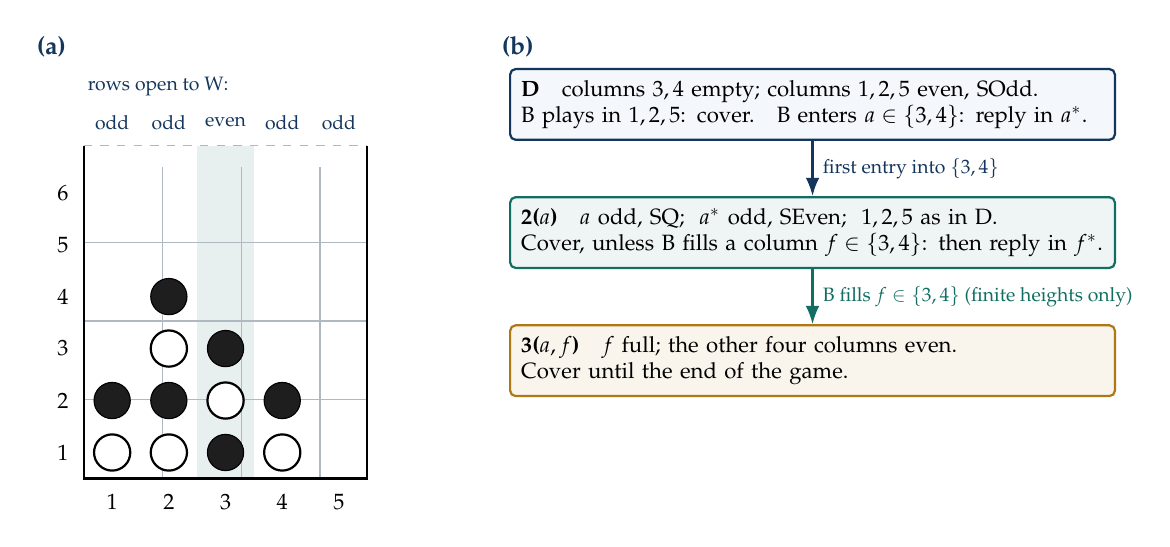
\begin{tikzpicture}[x=0.72cm,y=0.66cm,font=\footnotesize]
  % (a) the strip invariant
  \begin{scope}
    \node[anchor=west,font=\bfseries\small,text=primary] at (-1.0,8.3) {(a)};
    \fill[accent!10] (2,0) rectangle (3,6.4);
    \draw[gridgray] (0,0) grid (5,6);
    \draw[thick] (0,6.4) -- (0,0) -- (5,0) -- (5,6.4);
    \draw[dashed,gridgray] (0,6.4) -- (5,6.4);
    \foreach \c in {1,...,5} \node at (\c-0.5,-0.45) {\c};
    \foreach \r in {1,...,6} \node[anchor=east] at (-0.1,\r-0.5) {\r};
    \node[font=\scriptsize,text=primary,anchor=west] at (-0.1,7.55) {rows open to $\W$:};
    \foreach \c/\t in {1/odd,2/odd,3/even,4/odd,5/odd} \node[font=\scriptsize,text=primary] at (\c-0.5,6.85) {\t};
    \foreach \c/\r in {3/1,3/3,1/2,2/2,2/4,4/2} \node[bst] at (\c-0.5,\r-0.5) {};
    \foreach \c/\r in {3/2,1/1,2/1,2/3,4/1} \node[wst] at (\c-0.5,\r-0.5) {};
  \end{scope}
  % (b) the phases of the second player
  \begin{scope}[xshift=5.4cm]
    \node[anchor=west,font=\bfseries\small,text=primary] at (-0.3,8.3) {(b)};
    \node[draw=primary,thick,fill=softbg,rounded corners=2pt,text width=7.4cm,inner sep=4pt,anchor=north west] (d) at (0,7.9)
      {\textbf{D}\quad columns $3,4$ empty; columns $1,2,5$ even, $\mathrm{SOdd}$.\\
       $\B$ plays in $1,2,5$: cover.\quad $\B$ enters $a\in\{3,4\}$: reply in $a^*$.};
    \node[draw=accent,thick,fill=accent!7,rounded corners=2pt,text width=7.4cm,inner sep=4pt,below=7mm of d] (two)
      {\textbf{2($a$)}\quad $a$ odd, $\mathrm{SQ}$;\ \ $a^*$ odd, $\mathrm{SEven}$;\ \ $1,2,5$ as in D.\\
       Cover, unless $\B$ fills a column $f\in\{3,4\}$: then reply in $f^*$.};
    \node[draw=gold,thick,fill=gold!8,rounded corners=2pt,text width=7.4cm,inner sep=4pt,below=7mm of two] (three)
      {\textbf{3($a,f$)}\quad $f$ full; the other four columns even.\\
       Cover until the end of the game.};
    \draw[-{Latex},thick,primary] (d.south) -- node[right,font=\scriptsize]{first entry into $\{3,4\}$} (two.north);
    \draw[-{Latex},thick,accent] (two.south) -- node[right,font=\scriptsize]{$\B$ fills $f\in\{3,4\}$ (finite heights only)} (three.north);
  \end{scope}
\end{tikzpicture}
\caption{(a) The invariant of \cref{prop:inf-black} at a turn of $\W$, after the moves $3\,3\,3\,1\,1\,2\,2\,2\,2\,4\,4$. Column $3$ has odd height and stones of $\W$ only on even rows; the other columns have even height and stones of $\W$ only on odd rows. (b) The three phases of the second player's strategy (\cref{prop:white-even}). On the ceiling-free strip the game never leaves phase D or phase~2.}
\label{fig:easy}
\end{figure}

\subsection{The second player: pairing columns 3 and 4}

The second player cannot copy this strategy, because $\B$ may take the centre first. Instead $\W$ splits the columns into the \emph{ordinary} columns $U=\{1,2,5\}$ and the \emph{special pair} $P=\{3,4\}$, and writes $a^*$ for the other column of the pair ($3^*=4$, $4^*=3$). This is a pairing strategy in the style of Allis's rules \cite{allis1988}: the first stone of $\B$ in the pair is answered at the foot of the other column of the pair, and everything else is covered.

\begin{proposition}
\label{prop:white-even}
On the ceiling-free strip, and at every even height $h\ge 2$, $\W$ never loses by the following strategy.
\begin{itemize}
  \item As long as columns $3$ and $4$ are empty, cover every move. When $\B$ first plays in a column $a\in P$, play in $a^*$.
  \item After that, cover every move, except when the move of $\B$ fills a column $f\in P$. Then play in $f^*$, and cover every move from then on.
\end{itemize}
\lean{C4W5Inf.white_nonloss_inf, FiveAllis.white_nonloss_five}
\end{proposition}

\begin{proof}
\emph{The phases.} At every turn of $\B$ the position is in one of three phases (\cref{fig:easy}(b)).
\begin{itemize}[leftmargin=4.2em,labelwidth=3.6em,labelsep=0.6em,align=left]
  \item[D:] columns $3$ and $4$ are empty; every ordinary column has even height and pattern $\mathrm{SOdd}$.
  \item[2($a$):] column $a\in P$ has odd height and pattern $\mathrm{SQ}$; column $a^*$ has odd height and pattern $\mathrm{SEven}$; the ordinary columns are as in phase D.
  \item[3($a,f$):] column $f\in P$ is full and keeps its pattern from phase~2 ($\mathrm{SQ}$ if $f=a$, $\mathrm{SEven}$ if $f=a^*$); the other four columns have even height; the ordinary columns have pattern $\mathrm{SOdd}$; column $g=f^*$ is non-empty, has pattern $\mathrm{SOpen}$ and a stone of $\W$ on top; and if $f=a$, the stone of $g$ in row $1$ is not black.
\end{itemize}

\emph{The phases are maintained.} A stone of $\B$ in a column of even height lands on an odd row, and one in a column of odd height lands on an even row. Hence a move of $\B$ in an ordinary column keeps $\mathrm{SOdd}$, and in phase~2 a move in $a$ or in $a^*$ keeps $\mathrm{SQ}$ or $\mathrm{SEven}$; the cover of $\W$ restores the parities of the heights. In phase D, the first stone of $\B$ in $a\in P$ lies in row $1$, which $\mathrm{SQ}$ allows, and the reply of $\W$ in $a^*$ gives phase 2($a$).

In phases D and~2 the ordinary columns have even height at the turn of $\B$, so with an even ceiling $\B$ can fill only a column of $P$ of height $h-1$, which happens only in phase~2. Its stone then lies in row $h$, which is even, so the column keeps its pattern. The other column $g=f^*$ of the pair has odd height below $h$, so the reply in $g$ is legal; afterwards $g$ has even height, a stone of $\W$ on top, and pattern $\mathrm{SOpen}$, because $\mathrm{SQ}$ and $\mathrm{SEven}$ imply $\mathrm{SOpen}$. If $f=a$ then $g=a^*$ had pattern $\mathrm{SEven}$, so its stone in row $1$ is not black. This is phase 3($a,f$). In phase~3 every column that is not full has even height at the turn of $\B$, so no move of $\B$ fills a column and every cover is legal. A stone of $\B$ in $g$ lands on a stone of $\W$ and is covered at once, so $g$ keeps $\mathrm{SOpen}$ and its white top. On the ceiling-free strip no column is ever filled, and the game stays in phase D or phase~2.

\emph{No four of $\B$.} After each move of $\B$ the position satisfies:
(i) columns $1$, $2$ and $5$ have pattern $\mathrm{SOdd}$;
(ii) columns $3$ and $4$ have pattern $\mathrm{SOpen}$;
(iii) one of columns $3$ and $4$ has no black stone on an odd row $\ge 3$ (in phases D and~2 both, in phase~3 the column $f$);
(iv) one of columns $3$ and $4$ has no black stone in row $1$ (in phase D both; in phase~2 the column $a^*$; in phase 3 the column $f$ if $f=a^*$, and $g$ if $f=a$).
Under (i)--(iv), $\B$ has no four. Vertically, by (i) and (ii), no column holds three black stones in consecutive rows. Horizontally, every line contains columns $2$, $3$ and $4$ in one row $r$: if $r$ is even, column $2$ has no black stone there by (i); if $r\ge 3$ is odd, use (iii); if $r=1$, use (iv). Diagonally, a line in $W_0$ meets columns $1$ and $2$ in adjacent rows, and a line in $W_1$ meets columns $2$ and $5$ in rows that differ by $3$; in both cases one of the two rows is even, and both columns have pattern $\mathrm{SOdd}$.
\end{proof}

The parity regime explains why one reply suffices at even heights. With $\B$ to move, the number of empty cells is even ($\eps=0$ for the second player). In phase~2 the two special columns have odd remainders and the three ordinary columns even ones, so $\B$ can fill only a special column, and the reply in its partner leaves every remaining column with an even number of empty cells. From then on $\B$ can never fill a column again.

% ===== sec4_tools.tex =====
\section{Four reductions}
\label{sec:tools}

The remaining three subproblems need computer search, but a search over all positions of all heights is impossible. This section develops four reductions that turn each of them into finitely many finite checks. Throughout, the \emph{defender} is the player whose non-loss we prove and the \emph{attacker} is the other player; positions are considered at the attacker's turn. A column's \emph{remainder} is its number of empty cells. A move \emph{fills} a column if it puts a stone into the column's last empty cell.

The first three reductions are stated for either colour and are formalized in that generality in the namespace \code{C4W5Gen}, which was written for the odd heights. The proof for the first player at even heights was formalized earlier with versions specialized to $\B$ as defender (\code{C4W5.exists_exceptional_in_line}, \code{C4W5.claim_safe}, \code{C4W5.zone_safeL}), which are instances of the same statements. Stretching is used only for the first player at even heights and is formalized for that case.

\subsection{Shift-down}
\label{sec:shiftdown}

\begin{definition}
\label{def:exceptional}
A stone of the attacker is \emph{exceptional} if it lies in row $1$ or directly on another stone of the attacker. A \emph{potential exceptional cell} is the lowest empty cell of a column that is not full and is either empty or has a stone of the attacker on top.
\leanref{ExceptionalP, PotExcP}
\end{definition}

A potential exceptional cell is a cell where the attacker's next stone would be exceptional.

\begin{lemma}[Shift-down]
\label{lem:shiftdown}
If the defender has no four, then every four of the attacker contains an exceptional stone.
\lean{C4W5Gen.exists_exceptional_in_line_gen}
\end{lemma}

\begin{proof}
If no stone of a four of the attacker is exceptional, each of its four stones lies above row $1$ on a stone of the defender. Those four stones of the defender lie on the same line moved down by one row, so the defender has a four.
\end{proof}

The lemma becomes a strategy principle when the defender covers.

\begin{lemma}[Covering]
\label{lem:covering}
Let $R$ be a position with the attacker to move. Suppose that from $R$ on, the defender covers every move of the attacker that does not fill its column, and answers a move that fills a column anywhere. Then at every later turn of the attacker, every exceptional stone lies on a cell that held an exceptional stone or was a potential exceptional cell in $R$, and every potential exceptional cell was a potential exceptional cell in $R$.
\end{lemma}

\begin{proof}
Let $S$ be the set of cells that hold exceptional stones or are potential exceptional cells. A stone of the defender never adds a cell to $S$, because the cell above it is not a potential exceptional cell. A stone of the attacker placed outside $S$ lies on a stone of the defender and is not exceptional. Wherever the attacker plays, the cell above its stone may become a potential exceptional cell, but the defender covers that cell at once, unless the move filled the column, in which case there is no such cell. So after each pair of moves $S$ can only shrink.
\end{proof}

In Lean this argument is part of the invariant of the claim theorem (\code{C4W5Gen.cinvGen_step}) and of the zone discipline below. Together, the two lemmas say: as long as the defender covers, every new four of the attacker must pass through one of finitely many cells that are known in advance. Vertical fours need a separate but easy argument, because covering interrupts every vertical run of the attacker.

\subsection{Claims and the parity regime}
\label{sec:claims}

\begin{definition}
\label{def:claims}
Let $Q$ be a set of columns of a position $R$. The \emph{claimed cells} of a column $q\in Q$ are its empty cells in rows $|R(q)|+2,\ |R(q)|+4,\ \ldots$, that is, every second empty cell starting with the second. A non-vertical line of four cells is \emph{dead} if one of its cells holds a stone of the defender, is a claimed cell, or lies outside the board.
\leanref{ClaimedSet, LineOKSet}
\end{definition}

If the defender covers every move in $q$ and never enters $q$ on its own, then the attacker takes the first, third, fifth\,\dots\ empty cell of $q$ and the defender takes the claimed cells. The only danger is a forced reply after the attacker fills a column, and here the parity $\eps$ of \cref{sec:why5} decides which sets $Q$ can be held.

\begin{theorem}[Claims]
\label{thm:claims}
Let $R$ be a valid position with the attacker to move, in which neither player has a four and no column that is not full has three stones of the attacker on top. Suppose that one of the following holds.
\begin{itemize}[leftmargin=4.2em,labelwidth=3.6em,labelsep=0.6em,align=left]
  \item[(odd)] $\eps=1$, and $Q=\{q\}$ for a column $q$ with an odd remainder.
  \item[(even)] $\eps=0$, and $Q$ is the set of all columns that are not full and have an even remainder.
\end{itemize}
If every non-vertical line through an exceptional stone or a potential exceptional cell of $R$ is dead, then the defender does not lose from $R$. A strategy is: cover every move that does not fill its column; after a move that fills a column, play in a column that is not full and has no empty claimed cell.
\lean{C4W5Gen.claim_odd_safe, C4W5Gen.claim_even_safe}
\end{theorem}

\begin{proof}
\emph{The reply after a filling move exists.} At every turn of the attacker the number of empty cells has parity $\eps$, and every column of $Q$ that still has claimed cells has the same parity of remainder as in $R$, since only covers are played in it. Suppose the attacker fills a column $c$, leaving an even number of empty cells if $\eps=1$ and an odd number if $\eps=0$. In the even regime the columns of $Q$ have even remainders, so the columns outside $Q$ have an odd total remainder and one of them is not full. In the odd regime, if $c=q$ then $q$ is full and any column that is not full will do; otherwise $q$ has an odd remainder, so the other columns have an odd total and one of them is not full. (If no column at all is left, the board is full and the game is a draw.) This is the only place where the parity is used.

\emph{Claimed cells go to the defender.} The defender plays in a column of $Q$ only to cover. So the stones added to such a column alternate between the attacker and the defender, starting with the attacker, and the claimed cells receive stones of the defender. In the even regime a column of $Q$ has an even remainder at every turn of the attacker, so its last cell is claimed and the attacker never fills it. In the odd regime the last cell of $q$ is not claimed, and the attacker may fill it.

\emph{No vertical four.} At every turn of the attacker, a column that is not full has at most two stones of the attacker on top: this holds in $R$, and after any move of the attacker the defender covers it, unless the move filled the column.

\emph{No other four.} By \cref{lem:covering}, every exceptional stone at a later time lies on a cell that was exceptional or potentially exceptional in $R$. Suppose the attacker completes a non-vertical four. The defender has no four at that moment (otherwise the game would have ended), so by \cref{lem:shiftdown} the four contains an exceptional stone, and it is one of the lines through such a cell of $R$. That line was dead in $R$ and is still dead: stones of the defender stay, claimed cells receive stones of the defender, and cells outside the board stay outside. A dead line is not a four of the attacker.
\end{proof}

An odd value of $\eps$ does not mean that exactly one column has odd remainder: the count may be $1$, $3$ or $5$. The odd-regime theorem chooses a particular column $q$ whose remainder is odd and whose line-blocking hypotheses hold. The two regimes are exactly the ones in which the reply after a filling move can avoid the claimed columns. If $\eps=1$ and the defender claimed every column with an even remainder, a filling move could leave only claimed columns open. If $\eps=0$ and the defender claimed a single column with an odd remainder, a filling move could leave only that column open. This is why the second player at even heights and the first player at odd heights can afford to claim many columns at once, while in the other two cases only one column can be claimed.

\begin{example}
\label{ex:claim-h3}
Let $\B$ open in column $2$ on the $5\times 3$ board. With $\W$ to move, $\eps=(3+1)\bmod 2=0$. Column $2$ has remainder $2$ and the other columns have remainder $3$, so $Q=\{2\}$ and the claimed cell is row $3$ of column $2$. There are no white stones, and the potential exceptional cells are the bottom cells of columns $1$, $3$, $4$ and $5$. A horizontal line through row $1$ contains the black stone in column $2$, and a diagonal line needs four rows and leaves the board. So all relevant lines are dead and $\B$ does not lose. The same argument works on the $5\times 1$ board. These are the cases $H=1,3$ of \cref{sec:odd-black}; Lean checks the hypotheses of \cref{thm:claims} by evaluation \leanref{safeP_of_claimEven_run}.
\end{example}

\subsection{Zones}
\label{sec:zones}

Claims settle a position only when all danger is visible at once. Zones handle positions in which a fight is still going on, but only near the floor. Fix integers $K$ and $H$ with
\[
  K\equiv H \pmod 2\qquad\text{and}\qquad K+2\le H.
\]

\begin{definition}
\label{def:zone}
A position satisfies the \emph{zone discipline} for $K$ if every exceptional stone and every potential exceptional cell lies in row $K-3$ or below. The \emph{abstraction} of a position $R$ of height $H$ consists of its bottom $K$ rows together with a label for each column: a column of height $t$ is \emph{low} if $t\le K$, \emph{odd} if $t>K$ and $H-t$ is odd, and \emph{dead} if $t>K$ and $H-t$ is even.
\leanref{DiscEP, TColP, truncG, labOfG}
\end{definition}

\begin{lemma}
\label{lem:zone-low}
Under the zone discipline, if the defender has no four, every four of the attacker lies in the bottom $K$ rows.
\lean{C4W5Gen.oppFour_low}
\end{lemma}

\begin{proof}
By \cref{lem:shiftdown} the four contains an exceptional stone, which lies in row $K-3$ or below, and a four spans at most four consecutive rows.
\end{proof}

So above row $K$ only the labels matter. The \emph{zone game} is played on abstractions, with the attacker to move. The attacker may play:
\begin{itemize}
  \item in a low column below row $K$. The defender then answers with a stone in the bottom $K$ rows, or moves a low column of height $K$ out of the zone (its label becomes odd), or plays in an odd column (its label becomes dead). The defender may answer away from the attacker's column only if the attacker's stone lies in row $K-4$ or below.
  \item in a low column of height $K$. The defender covers, and the label becomes dead.
  \item in an odd column. If the move does not fill the column, the defender covers and nothing changes. If it fills the column, the label becomes dead and the defender answers as in the first case.
  \item in a dead column. The move cannot fill the column (its remainder is even and positive), the defender covers, and nothing changes.
\end{itemize}
A \emph{zone certificate} for $K$ is a finite set of abstractions that is closed under this game: for each member and each move of the attacker, the attacker completes no four in the bottom $K$ rows, and the certificate names a reply of the defender that completes a four of the defender, leads back into the set, or leads to a \emph{leaf}. A leaf is an abstraction from which non-loss is known by another argument; in this paper every leaf is a position satisfying the hypotheses of \cref{thm:claims} on the board of height $K$. A certificate may also end when every column is above the zone.
\leanref{ZoneCert2P}

\begin{theorem}[Zones]
\label{thm:zones}
Let $K\equiv H \pmod 2$ and $K+2\le H$, and let $I$ be a zone certificate for $K$. If $R$ is a valid position of height $H$ with the attacker to move, in which neither player has a four, which satisfies the zone discipline for $K$, and whose abstraction belongs to $I$, then the defender does not lose from $R$. The same certificate therefore serves for every height $H\equiv K\pmod 2$ with $H\ge K+2$.
\lean{C4W5Gen.zone_safeL_gen}
\end{theorem}

\begin{proof}
The defender plays the certificate's replies for moves in the zone and for moves that fill an odd column, and covers every other move. Once every column is above row $K$ it covers, and answers a filling move anywhere. We check that the zone discipline is kept, that the labels change as in the zone game, and that the attacker never completes a four.

\emph{Labels.} The certificate does not know $H$, and the parity condition is what makes this harmless. A column that leaves the zone has $K+1$ stones and $H-K-1$ empty cells, an odd number; after the cover it has $K+2$ stones and an even remainder. Covering a move in an odd column keeps its label, and filling it leaves zero empty cells, so the label becomes dead. The condition $K+2\le H$ makes every cover above the zone legal.

\emph{Discipline.} A stone of the defender never creates an exceptional stone or a potential exceptional cell. A stone of the attacker on a potential exceptional cell is exceptional, but such a cell lies in row $K-3$ or below. A stone of the attacker that is not covered leaves a potential exceptional cell directly above it; the zone game allows this only when the stone lies in row $K-4$ or below, so the new cell lies in row $K-3$ or below.

\emph{Fours.} By \cref{lem:zone-low}, every four of the attacker lies in the bottom $K$ rows, which the abstraction records exactly, and the certificate excludes such fours. Once every column is above row $K$ the bottom $K$ rows no longer change, so no four can appear. When the play reaches a leaf, \cref{thm:claims} applies to the real position: every line through an exceptional stone or a potential exceptional cell lies in rows $1$ to $K$, so a line that is dead on the board of height $K$ is dead on the board of height $H$ \leanref{claimOdd_zoneLeafSound, claimEven_zoneLeafSound}.
\end{proof}

Together with claims, zones decide all odd heights (\cref{sec:odd}). At even heights for the first player they are not enough: along the main line of \cref{sec:even-black}, $\W$ can build an alternating wall in column $2$ that grows with the height and leaves every fixed zone.

\subsection{Clear-cut stretching}
\label{sec:stretch}

A \emph{level} $\ell\in\{0,\dots,h\}$ of a board of height $h$ is the boundary between rows $\ell$ and $\ell+1$. A column has a \emph{defect} at level $\ell$ if its stones in rows $\ell$ and $\ell+1$ exist and have the same colour. The \emph{landmarks} of a position are the levels $0$ and $h$, the heights of its columns, and the levels of its defects. Away from the landmarks every column is either empty or alternates in colour.

\begin{definition}
\label{def:clearcut}
A level $r$ is a \emph{clear cut of radius $D$} of a position $A$ of height $h$ if $r\le h$ and every landmark $\ell$ satisfies $|\ell-r|>D$. \emph{Stretching} $A$ at $r$ inserts two stones above row $r$ in every column taller than $r$: the new rows $r+1$ and $r+2$ repeat the colours of rows $r+1$ and $r$, and the old rows $r+1,r+2,\dots$ move up by two. Columns of height below $r$ are unchanged, and the ceiling rises to $h+2$. We write $\mathrm{stretch}(A,r)$ for the result, and say that $R$ is a \emph{stretch} of $A$ if it arises from $A$ by finitely many stretches, each at a clear cut of the board it is applied to.
\leanref{Landmark, ClearCut, stretch, SEq}
\end{definition}

Since every column through a clear cut alternates near it, stretching inserts one more alternating pair; see \cref{fig:stretch}. If no column reaches the cut, stretching only raises the ceiling. All computations in this paper use $D=2$.

\begin{figure}[!htbp]
\centering
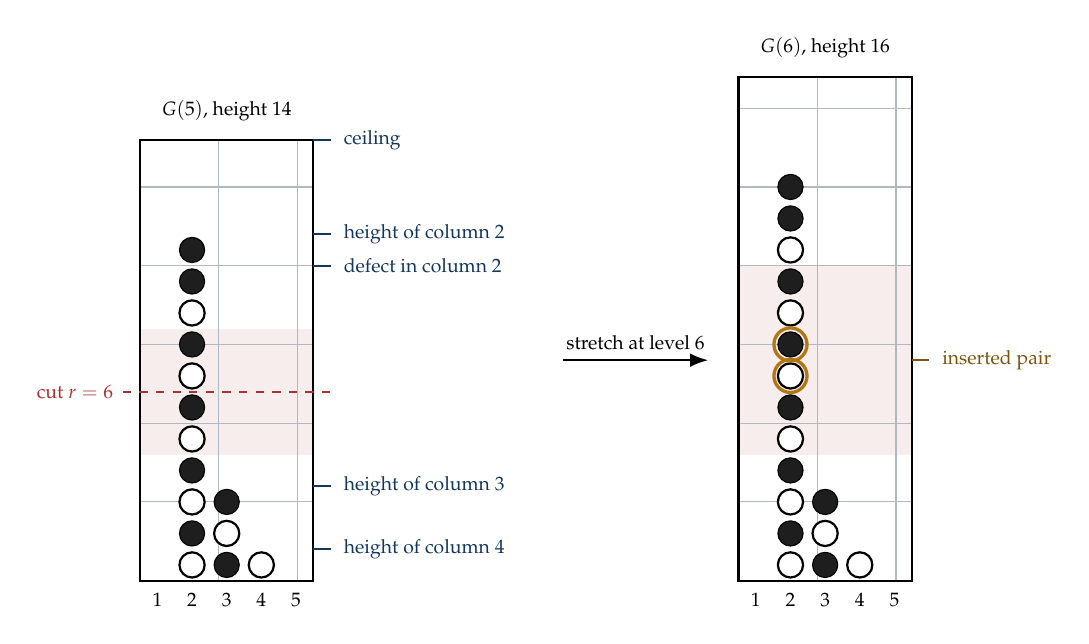
\begin{tikzpicture}[x=0.44cm,y=0.40cm,font=\scriptsize,
  bs/.style={circle,fill=stoneB,draw=black,inner sep=0pt,minimum size=3.2mm},
  ws/.style={circle,fill=white,draw=black,thick,inner sep=0pt,minimum size=3.2mm},
  ins/.style={circle,draw=gold,very thick,inner sep=0pt,minimum size=4.2mm}]
  % left board: G(5) on 5 x 14
  \begin{scope}
    \fill[warn!9] (0,4) rectangle (5,8);
    \draw[gridgray] (0,0) grid (5,14);
    \draw[thick] (0,14) -- (0,0) -- (5,0) -- (5,14) -- cycle;
    \draw[warn,thick,dashed] (-0.5,6) -- (5.5,6);
    \node[warn,anchor=east] at (-0.5,6) {cut $r=6$};
    \foreach \c in {1,...,5} \node at (\c-0.5,-0.6) {\c};
    \foreach \p [count=\r] in {w,b,w,b,w,b,w,b,w,b,b} {\node[\p s] at (1.5,\r-0.5) {};}
    \node[bs] at (2.5,0.5) {}; \node[ws] at (2.5,1.5) {}; \node[bs] at (2.5,2.5) {};
    \node[ws] at (3.5,0.5) {};
    \foreach \l/\t in {14/{ceiling},11/{height of column 2},10/{defect in column 2},3/{height of column 3},1/{height of column 4}}
      {\draw[primary,thick] (5,\l) -- (5.5,\l); \node[primary,anchor=west] at (5.6,\l) {\t};}
    \node[anchor=south] at (2.5,14.3) {$G(5)$, height $14$};
  \end{scope}
  \draw[-{Latex},thick] (12.2,7) -- node[above]{stretch at level $6$} (16.4,7);
  % right board: G(6) on 5 x 16
  \begin{scope}[xshift=7.6cm]
    \fill[warn!9] (0,4) rectangle (5,10);
    \draw[gridgray] (0,0) grid (5,16);
    \draw[thick] (0,16) -- (0,0) -- (5,0) -- (5,16) -- cycle;
    \foreach \c in {1,...,5} \node at (\c-0.5,-0.6) {\c};
    \foreach \p [count=\r] in {w,b,w,b,w,b,w,b,w,b,w,b,b} {\node[\p s] at (1.5,\r-0.5) {};}
    \node[ins] at (1.5,6.5) {}; \node[ins] at (1.5,7.5) {};
    \node[bs] at (2.5,0.5) {}; \node[ws] at (2.5,1.5) {}; \node[bs] at (2.5,2.5) {};
    \node[ws] at (3.5,0.5) {};
    \draw[gold!70!black,thick] (5,7) -- (5.5,7); \node[gold!70!black,anchor=west] at (5.6,7) {inserted pair};
    \node[anchor=south] at (2.5,16.3) {$G(6)$, height $16$};
  \end{scope}
\end{tikzpicture}
\caption{Stretching at a clear cut. Left: the position $G(5)$ of \cref{sec:even-black} on a board of height $14$. Its landmarks are the levels $0$, $1$, $3$, $10$, $11$ and $14$ (the defect at level $10$ is the pair of black stones in rows $10$ and $11$ of column $2$), so level $6$ is a clear cut of radius $2$; the shaded band contains the levels within distance $2$ of the cut. Right: stretching at level $6$ inserts the pair marked in gold into column $2$ and raises the ceiling by two. The result is $G(6)$ on a board of height $16$.}
\label{fig:stretch}
\end{figure}

\begin{lemma}[Fours are preserved]
\label{lem:stretchA}
Let $D\ge 2$, let $r$ be a clear cut of radius $D$ of a position $A$ of height $h$, and let $A'=\mathrm{stretch}(A,r)$. For both players $p$, $A$ has a four of $p$ if and only if $A'$ (of height $h+2$) has one.
\lean{C4W5.hasFour_stretch_iff}
\end{lemma}

\begin{proof}
Since $r$ is a clear cut, every column either ends below level $r-D$, or passes level $r+D$ and has no defect between levels $r-D$ and $r+D$. This gives two facts about single cells:
\begin{itemize}
  \item[(a)] $A'$ and $A$ agree on rows $1,\dots,r+D+1$;
  \item[(b)] row $y$ of $A'$ agrees with row $y-2$ of $A$ for every $y\ge r-D+2$.
\end{itemize}
Fact (b) holds above the inserted pair by construction, and inside the band because an alternating column has the same colour two rows apart; fact (a) holds for the same reason. Since $h$ is a landmark, $r+D<h$, so the rows in (a) lie on both boards. A four occupies at most four consecutive rows, say rows $y_0$ to $y_0+3$. If $y_0+3\le r+D+1$, fact (a) transfers it between $A$ and $A'$. Otherwise $y_0\ge r+D-1$, and $r+D-1\ge r-D+2$ because $D\ge 2$; fact (b) then transfers the four, moved by two rows. In the direction from $A$ to $A'$ already $D\ge1$ suffices, but from $A'$ to $A$ the radius $D=1$ fails: a four of $A'$ in rows $r$ to $r+3$ would be covered by neither fact.
\end{proof}

When a stone is added to a column of height $t$, a new landmark appears at level $t+1$. A clear cut $r$ of $A$ stays clear unless $|r-(t+1)|\le D$, and since $|r-t|>D$ this happens only for $r=t+D+1$. Stretching commutes with the move at every cut that stays clear. The one exception gives two possible abstract images of a real move.

\begin{lemma}[Moves]
\label{lem:stretchB}
Let $R$ (of height $H$) be a stretch of $A$ (of height $h$), and let a stone of colour $p$ be played in column $c$. Then $\mathrm{play}(R,c,p)$ is a stretch of $\mathrm{play}(A,c,p)$ (of height $h$), or the level $r^\ast=|A(c)|+D+1$ is a clear cut of $A$ while $r^\ast+1$ is not, and $\mathrm{play}(R,c,p)$ is a stretch of $\mathrm{play}(\mathrm{stretch}(A,r^\ast),c,p)$ (of height $h+2$). We call these the \emph{variants} of the move.
\lean{C4W5.SEq.play, C4W5.exists_variant}
\end{lemma}

\begin{proof}[Proof sketch]
Induct on the number of stretches. A stretch at a cut $r\ne r^\ast$ commutes with the move. If $R$ contains a stretch at $r^\ast$ and $r^\ast+1$ is also a clear cut, then stretching at $r^\ast$ and at $r^\ast+1$ gives the same board, because the columns alternate at both levels, so the stretch can be moved to $r^\ast+1$, which survives the move. Otherwise the stretch at $r^\ast$ is performed on $A$ before the move, which is the second variant.
\end{proof}

\begin{theorem}[Stretching]
\label{thm:stretch}
Let $D\ge 2$ and let $I$ be a set of positions $(h,A)$ with $\W$ to move. Suppose that for every $(h,A)\in I$, every legal move $c$ of $\W$ and every variant $(h_1,A_1)$ of it, $\W$ has no four in $A_1$, and either $A_1$ is full or $\B$ has a legal move $e$ such that every variant $(h_2,A_2)$ of $e$ either contains a four of $\B$ or is a stretch of a member of $I$ or of a leaf. Then $\B$ does not lose from any position with $\W$ to move and no four of $\W$ that is a stretch of a member of $I$.
\lean{C4W5.stretch_safe, C4W5.stretch_safeL}
\end{theorem}

\begin{proof}
By \cref{lem:stretchB}, the real position after each move is a stretch of one of the variants, which the hypothesis covers. By \cref{lem:stretchA}, fours correspond, and legality and fullness correspond because stretching changes no column's status of being full \leanref{SEq.legal_iff, SEq.full_iff}. Induction on the horizon $k$ of $\SafeFor$ completes the proof.
\end{proof}

A finite set $I$ thus covers infinitely many real positions. An alternating wall $(\W\B)^b$ contains no landmark, so the positions for all large $b$ are stretches of one of them; stretching at a level above every column raises only the ceiling, so one position covers all larger heights.

The last tool combines stretching with zones. A \emph{zone-on-stretch certificate} is a set of abstractions $(k,A,\ell)$, each with its own zone height $k$, closed under the zone game in which every move of the bottom $k$ rows is played in all its variants and membership is tested up to stretching. Its stretches to a common zone height $K$ form a zone certificate for $K$.

\begin{theorem}[Zone on stretch]
\label{thm:sz}
A zone-on-stretch certificate yields, for every $K$, a zone certificate for $K$ whose members are the stretches of its members to zone height $K$. Consequently, for even $K$, \cref{thm:zones} applies with $\B$ as defender at every even height $H\ge K+2$.
\lean{C4W5.zoneCert2_of_sz, C4W5.sz_safe}
\end{theorem}

In \cref{sec:even-black} one such certificate, built at zone height $14$, covers a two-parameter family of positions whose zone height grows with the parameter.

% ===== sec5_odd.tex =====
\section{Odd heights}
\label{sec:odd}

At odd heights claims and zones suffice; stretching is not needed. All certificates for odd heights together store $142{,}219$ positions (\cref{tab:odd-certs}).

\subsection{The first player}
\label{sec:odd-black}

The first player opens in column $2$ at every odd height. With $\W$ to move after this move, $\eps=(H+1)\bmod 2=0$, so $\B$ is in the regime where every column with an even remainder can be claimed.

\paragraph{Why column 2.} After $\B_2$, column $2$ has odd height and column $4$ even height. As long as $\B$ covers, stones of $\W$ in column $2$ land on even rows and stones of $\W$ in column $4$ on odd rows. Every non-vertical line meets both columns $2$ and $4$, and in rows of the same parity: the same row for a horizontal line, rows two apart for a diagonal one. So no such line can be completed by $\W$, and vertical lines are stopped by covering. This breaks down only when $\W$ fills a column and $\B$ has to reply elsewhere. The replies to such moves below were found by search; they use column $4$ only as a last resort.

\paragraph{The strategy.} The proof is split by height.
\begin{itemize}
  \item $H=1$ and $H=3$: the position after $\B_2$ satisfies the claim theorem directly (\cref{ex:claim-h3}).
  \item $H=5$: a finite certificate with $324$ positions, ending in claim leaves.
  \item $H=7$, and every odd $H\ge 9$: a fixed controller. If $\B$ can complete a four, it does so (in the lowest-numbered such column). Otherwise, if the last move of $\W$ did not fill its column, $\B$ covers it. Otherwise $\W$ has just filled a column $c$, and $\B$ plays in the first column of the following list that is not full:
  \begin{center}
  \small
  \begin{tabular}{@{}ll@{}}
    $c=1$: & $3,\ 2,\ 5,\ 4$\\
    $c=3$: & $2$ if column $2$ holds at most $3$ stones and column $5$ at most $2$;\\
           & otherwise $5,\ 1,\ 2,\ 4$\\
    $c=5$: & $3,\ 1,\ 2,\ 4$\\
    $c\in\{2,4\}$:\ \ & $1,\ 3,\ 5,\ 2,\ 4$
  \end{tabular}
  \end{center}
  \leanref{oddBlackCap4Line, oddBlackRealReply}
\end{itemize}
For $H=7$ the controller is checked on the real board, and for all odd $H\ge 9$ at once in the zone game with $K=7$ (\cref{thm:zones}). The two certificates store the $947$ and $2{,}094$ positions that the controller can reach before an exit, and no replies. The kernel computes the controller's reply in each stored position and checks that every successor is stored, satisfies the claim theorem, or, in the zone game, leaves the zone. After such an exit the claim theorem or the zone theorem takes over; we do not claim that the controller itself is followed beyond the exits.

\begin{theorem}
\label{thm:odd-black}
At every odd height $h\ge 1$, the first player does not lose.
\lean{C4W5Gen.odd_black_nonloss}
\end{theorem}

\subsection{The second player}
\label{sec:odd-white}

With $\B$ to move at an odd height, $\eps=1$, so $\W$ can claim only one column. By mirror symmetry it suffices to answer the first moves $\B_1$, $\B_2$ and $\B_3$; the answers to $\B_4$ and $\B_5$ are the mirror images of those to $\B_2$ and $\B_1$ \leanref{safeP_mirror}. The replies of $\W$ in the opening are fixed:
\begin{center}
\small
\begin{tabular}{@{}lll@{}}
\toprule
first move of $\B$ & reply of $\W$ & then \\
\midrule
$\B_1$ & $\W_2$ & certificate \\
$\B_2$ & $\W_3$ (but $\W_2$ if $H=5$) & certificate; for $H\ge 9$ one more fixed reply: \\
 & & \quad $\B_1\W_3$, $\B_2\W_2$, $\B_3\W_3$, $\B_4\W_2$, $\B_5\W_3$ \\
$\B_3$ & $\W_2$ & certificate \\
\bottomrule
\end{tabular}
\end{center}

After these replies the proof is split by height.
\begin{itemize}
  \item $H=1$ and $H=3$: after the reply, the claim theorem applies directly (no stored positions).
  \item $H=5$ and $H=7$: three finite certificates each, for the openings $\B_1\W_2$, $\B_2\W_2$ or $\B_2\W_3$, and $\B_3\W_2$.
  \item $H=9$: five zone certificates with $K=7$, which hold at every odd $H\ge 9$, and two finite certificates for the continuations $\B_2\W_3\B_3\W_3$ and $\B_2\W_3\B_4\W_2$.
  \item odd $H\ge 11$: the same five zone certificates with $K=7$, and two zone certificates with $K=9$ for those two continuations.
\end{itemize}
The two continuations need $K=9$, and a zone certificate for $K=9$ applies only from $H=11$ on, since \cref{thm:zones} requires $K+2\le H$; the two finite certificates for $H=9$ fill exactly this gap.

\begin{theorem}
\label{thm:odd-white}
At every odd height $h\ge 1$, the second player does not lose.
\lean{C4W5Gen.odd_white_nonloss}
\end{theorem}

\paragraph{The switch at height 5.} On the $5\times5$ board the reply $\W_3$ to $\B_2$ loses: $\B$ wins after $\B_2\W_3$. This is why $\W$ answers $\B_2$ with $\W_2$ at height $5$. The other reply is not uniform either: an independent search (\cref{app:recheck}) shows that $\B$ also wins after $\B_2\W_2$ on the $5\times 9$ board. So neither of the two natural answers to $\B_2$ works at every odd height. We did not examine $\W_1$, $\W_4$ and $\W_5$.

\begin{table}[!htbp]
\centering
\caption{The $18$ certificate packages for odd heights. ``Positions'' counts stored positions; the two controller certificates store positions without replies. A chunk is a subtree of at most $512$ positions with its own kernel check. In total the packages form $114$ Lean modules.}
\label{tab:odd-certs}
\footnotesize
\begin{tabularx}{\linewidth}{@{}l l Y r r@{}}
\toprule
\textbf{Defender, scope} & \textbf{Package} & \textbf{Content} & \textbf{Positions} & \textbf{Chunks} \\
\midrule
$\B$, $H=5$ & \code{B5_B2} & tree after $\B_2$, claim leaves & 324 & 1 \\
$\B$, $H=7$ & \code{B7_B2_Explicit} & controller, real board & 947 & 2 \\
$\B$, odd $H\ge 9$ & \code{BZ7_B2_Explicit} & controller, zone game $K=7$ & 2{,}094 & 8 \\
\midrule
$\W$, $H=5$ & \code{W5_B1W2}, \code{W5_B2W2}, \code{W5_B3W2} & trees: $99+2{,}656+16$ & 2{,}771 & 10 \\
$\W$, $H=7$ & \code{W7_B1W2}, \code{W7_B2W3}, \code{W7_B3W2} & trees: $326+14{,}124+22$ & 14{,}472 & 34 \\
$\W$, $H=9$ & \code{W9_B2W3_B4W2}, \code{W9_B2W3_B3W3} & trees: $10{,}668+20{,}593$ & 31{,}261 & 96 \\
$\W$, odd $H\ge 9$ & \code{WZ7_*} (5 packages) & zone $K=7$: \code{B3W2} 28, \code{B1W2} 538, \code{B2W3_B1W3} 85, \code{B2W3_B2W2} 112, \code{B2W3_B5W3} 260 & 1{,}023 & 6 \\
$\W$, odd $H\ge 11$ & \code{WZ9_B2W3_B4W2} & zone $K=9$ & 30{,}602 & 64 \\
$\W$, odd $H\ge 11$ & \code{WZ9_B2W3_B3W3} & zone $K=9$ & 58{,}725 & 128 \\
\midrule
\multicolumn{3}{@{}l}{\textbf{Total} (first player $3{,}365$, second player $138{,}854$)} & \textbf{142{,}219} & \textbf{349} \\
\bottomrule
\end{tabularx}
\end{table}

% ===== sec6_even.tex =====
\section{Even heights: the first player}
\label{sec:even-black}

This is the hard case. With $\W$ to move at an even height, $\eps=1$, so $\B$ can claim only one column, and the defender must survive the replies forced by every filling move of $\W$.

\subsection{What small heights rule out}
\label{sec:counterexamples}

Exhaustive search on small boards constrains any strategy that is meant to work at every even height:
\begin{itemize}
  \item on the $5\times 4$ board, opening in column $1$ or column $5$ loses;
  \item on the $5\times 8$ board, opening in column $2$ loses: after $\B_2\W_2$ every move of $\B$ loses;
  \item on the $5\times 8$ board, after $\B_3\W_3$ the moves $\B_1$, $\B_2$, $\B_4$ and $\B_5$ lose, and only the cover $\B_3$ draws.
\end{itemize}
A first move that works at every even height must therefore be the centre, and the answer to $\W_3$ must be $\B_3$. These facts do not show that the line chosen below is forced for strategies that depend on the height, and they do not show that stretching is unavoidable.

\subsection{The opening and the main line}

The first player opens in the centre and covers the reply of $\W$, which gives \cref{cor:centre}. This leads to five positions, two of which are mirror images of two others:
\[
  P_{311}=\col{\W\B,\ \varnothing,\ \B,\ \varnothing,\ \varnothing},\qquad
  P_{322}=\col{\varnothing,\ \W\B,\ \B,\ \varnothing,\ \varnothing},\qquad
  T(0)=\col{\varnothing,\ \varnothing,\ \B\W\B,\ \varnothing,\ \varnothing},
\]
the positions after $311$, $322$ and $333$. In $T(0)$, $\B$ again covers each move of $\W$, except that it answers $\W_3$ with $\B_2$. The main line is the reply $\W_2$, after which $\W$ can keep playing in column $2$ and $\B$ keeps covering, building an alternating wall:
\[
  T(b)=\col{\varnothing,\ (\W\B)^b,\ \B\W\B,\ \varnothing,\ \varnothing}\qquad(\text{after } 333\,(22)^b,\ \W\text{ to move}).
\]
On the board of height $2m$ the wall can grow until $b=m-1$, when it ends two rows below the ceiling. \Cref{tab:spine} lists the reply of $\B$ to each move of $\W$ in $T(b)$; the positions it leads to are
\begin{align*}
  G(b) &= T(b)\cdot\W_4\B_2 = \col{\varnothing,\ (\W\B)^b\B,\ \B\W\B,\ \W,\ \varnothing},\\
  \Top(m) &= T(m-1)\cdot\W_2\B_4 = \col{\varnothing,\ (\W\B)^{m-1}\W,\ \B\W\B,\ \B,\ \varnothing},\\
  \Side(b,q) &= T(b)\cdot\W_q\B_4\qquad (q\in\{1,3,5\}),
\end{align*}
together with $T(1)\cdot\W_3\B_2$ and $T(2)\cdot\W_3\B_5$ (\cref{fig:spine}). Certificate names refer to positions by short labels: $U=T(0)\cdot\W_3\B_2$, $33311=T(0)\cdot\W_1\B_1$, $s113=T(1)\cdot\W_3\B_2$ and $s123=T(2)\cdot\W_3\B_5$.

\begin{table}[!htbp]
\centering
\caption{The replies of $\B$ on the main line, for $1\le b\le m-1$ on the board of height $2m$.}
\label{tab:spine}
\small
\begin{tabular}{@{}cll@{}}
\toprule
move of $\W$ in $T(b)$ & reply of $\B$ & resulting position \\
\midrule
$\W_1$ & $\B_4$ & $\Side(b,1)$ \\
$\W_2$ & $\B_2$ if $b<m-1$; \ $\B_4$ if $b=m-1$ & $T(b+1)$; \ $\Top(m)$ \\
$\W_3$ & $\B_2$ if $b=1$; \ $\B_5$ if $b=2$; \ $\B_4$ if $b\ge 3$ & $T(1)\W_3\B_2$; \ $T(2)\W_3\B_5$; \ $\Side(b,3)$ \\
$\W_4$ & $\B_2$ & $G(b)$ \\
$\W_5$ & $\B_4$ & $\Side(b,5)$ \\
\bottomrule
\end{tabular}
\end{table}

At the top of the wall $\B$ must not cover: on the boards of height $10$ and $12$, the position $T(m-1)\cdot\W_2\B_2$, in which $\B$ fills column $2$, is a win for $\W$ (\cref{app:recheck}). The reply $\B_4$ leads to $\Top(m)$ instead.

\begin{figure}[!htbp]
\centering
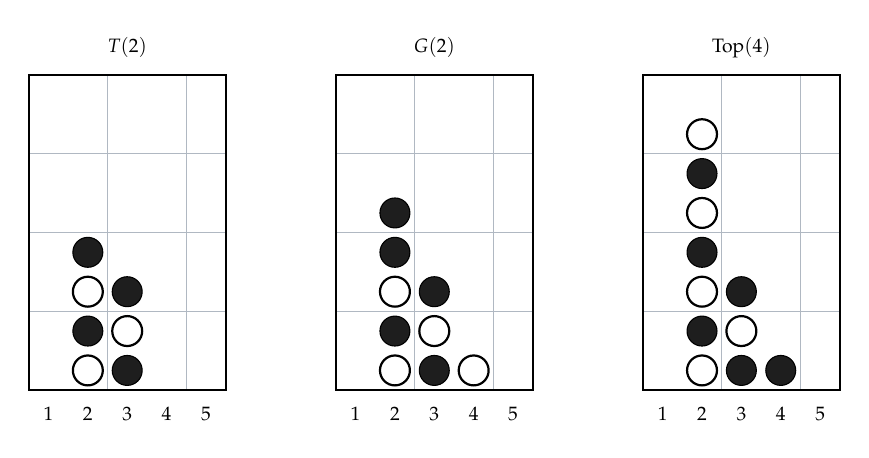
\begin{tikzpicture}[x=0.5cm,y=0.5cm,font=\scriptsize,
  bs/.style={circle,fill=stoneB,draw=black,inner sep=0pt,minimum size=3.8mm},
  ws/.style={circle,fill=white,draw=black,thick,inner sep=0pt,minimum size=3.8mm}]
  \foreach \X/\name/\two/\four in {
      0/{$T(2)$}/{w,b,w,b}/{},
      3.9/{$G(2)$}/{w,b,w,b,b}/{w},
      7.8/{$\Top(4)$}/{w,b,w,b,w,b,w}/{b}} {
    \begin{scope}[xshift=\X cm]
      \draw[gridgray] (0,0) grid (5,8);
      \draw[thick] (0,8) -- (0,0) -- (5,0) -- (5,8) -- cycle;
      \foreach \c in {1,...,5} \node at (\c-0.5,-0.6) {\c};
      \foreach \p [count=\r] in \two {\node[\p s] at (1.5,\r-0.5) {};}
      \node[bs] at (2.5,0.5) {}; \node[ws] at (2.5,1.5) {}; \node[bs] at (2.5,2.5) {};
      \foreach \p [count=\r] in \four {\node[\p s] at (3.5,\r-0.5) {};}
      \node[anchor=south] at (2.5,8.2) {\name};
    \end{scope}}
\end{tikzpicture}
\caption{Positions of the main line on the board of height $8$ ($m=4$), each with $\W$ to move: the spine position $T(2)$, the breakout $G(2)=T(2)\cdot\W_4\B_2$, and the top position $\Top(4)=T(3)\cdot\W_2\B_4$.}
\label{fig:spine}
\end{figure}

\subsection{How each position is closed}
\label{sec:coverage}

Every position in \cref{tab:spine}, and every first reply at $T(0)$, is closed by one of four methods: a finite certificate on the real board (``tree''), a zone certificate (\cref{thm:zones}), a stretch certificate (\cref{thm:stretch}), or a zone-on-stretch certificate (\cref{thm:sz}). \Cref{tab:coverage} gives the complete assignment, and \cref{fig:gwedge} shows the two-parameter family $G(b)$.

\begin{table}[!htbp]
\centering
\caption{How each position is closed on the board of height $H=2m$. Trees are finite certificates for one height; \code{Z}$K$ denotes a zone certificate for zone height $K$, valid for every even $H\ge K+2$; \code{S} denotes stretching. For $m\le 4$ the trees for $P_{311}$, $P_{322}$ and $T(0)$ cover everything below them.}
\label{tab:coverage}
\footnotesize
\begin{tabularx}{\linewidth}{@{}l l l l Y@{}}
\toprule
\textbf{Position} & $m\le 4$ & $m=5$ & $m=6$ & $m\ge 7$ \\
\midrule
empty board, $m=1$ & tree \code{H2} & & & \\
$P_{311}$ & trees \code{H4}--\code{H8} & tree \code{H10} & \code{Z10_311} & \code{Z10_311} \\
$P_{322}$ & trees \code{H4}--\code{H8} & \code{Z8_322} & \code{Z8_322} & \code{Z8_322} \\
$T(0)$ & trees \code{H4}--\code{H8} & main line & main line & main line \\
$T(0)\cdot\W_1\B_1$ & & \code{Z8_33311} & \code{Z8_33311} & \code{Z8_33311} \\
$T(0)\cdot\W_3\B_2$ & & tree \code{H10_U} & \code{Z10_U} & \code{Z10_U} \\
$\Side(b,q)$, $b\in\{1,2\}$, $q\in\{1,5\}$ & & \code{Z8_side}$bq$ & \code{Z8_side}$bq$ & \code{Z8_side}$bq$ \\
$T(1)\cdot\W_3\B_2$, \ $T(2)\cdot\W_3\B_5$ & & \code{Z8_s113}, \code{Z8_s123} & same & same \\
$\Side(b,q)$, $b\ge 3$ & & claim on column $4$ & same & same \\
$\Top(m)$ & & tree \code{H10_Top} & tree \code{H12_Top} & \code{STop}: stretch of $\Top(5)$ \\
$G(b)$ & & \multicolumn{3}{l}{see \cref{fig:gwedge}} \\
\bottomrule
\end{tabularx}
\end{table}

\paragraph{The side moves for $b\ge 3$.} After $\Side(b,q)$ with $b\ge 3$, $\B$ claims column $4$, which holds one stone and has the odd remainder $2m-1$. All exceptional white stones and potential exceptional cells lie in the bottom five rows, so the hypotheses of \cref{thm:claims} concern only the bottom eight rows. There the wall looks the same for every $b\ge 4$, so two finite checks, for $b=3$ and $b=4$, settle every $b\ge 3$ and every even height $H\ge 2b+2$. No strategy certificate is needed \leanref{C4W5.wall_family_safe}.

\paragraph{Stretching.} Four certificate families use \cref{lem:stretchA,lem:stretchB}, all with $D=2$:
\begin{itemize}
  \item \code{STop}: $\Top(m)$ on height $2m$ is a stretch of $\Top(5)$ on height $10$; the wall is stretched $m-5$ times at level $6$ \leanref{C4W5.seq_Top}. The build uses it for $m\ge 7$.
  \item \code{SG3}: $G(3)$ on height $14+2k$ is a stretch of $G(3)$ on height $14$, at a level above all columns, which only raises the ceiling \leanref{C4W5.seq_G3}.
  \item \code{SG5}: for $b\ge 5$, $G(b)$ on height $2b+2$ or $2b+4$, where the wall ends one or three rows below the ceiling, is a stretch of $G(5)$ on height $12$ or $14$ \leanref{C4W5.seq_G_wall}.
  \item \code{SGZ5R}: for $b\ge 5$ and $m\ge b+3$, the bottom $2b+4$ rows of $G(b)$ are a stretch of the bottom $14$ rows of $G(5)$. A single zone-on-stretch certificate rooted at $G(5)$ with zone height $14$ therefore covers zone height $K=2b+4$ and every height $2m\ge K+2$ (\cref{thm:sz}). Its compact table is the wide-gap endpoint \code{C4W5.SGZLongPacked.g5_wide}, whose complete shard set and endpoint are kernel-accepted.
\end{itemize}

\begin{figure}[!htbp]
\centering
\begin{tikzpicture}[x=0.78cm,y=0.62cm,font=\scriptsize]
  \tikzset{cell/.style={draw=white,thick}}
  \def\cellat#1#2#3#4{\fill[#3,cell] (#1-0.48,#2-0.46) rectangle (#1+0.48,#2+0.46); \node at (#1,#2) {#4};}
  % axes
  \foreach \b in {1,...,8} \node at (\b,1.2) {\b};
  \node at (4.5,0.55) {$b$};
  \foreach \m in {2,...,9} \node[anchor=east] at (0.4,\m) {\m};
  \node[anchor=east] at (-0.2,5.5) {$m$};
  % m <= 4: inside the direct 333 trees
  \foreach \m in {2,3,4} {\pgfmathtruncatemacro\top{\m-1}
    \foreach \b in {1,...,\top} {\cellat{\b}{\m}{black!12}{}}}
  % m = 5
  \cellat{1}{5}{accent!30}{Z8}
  \foreach \b in {2,3,4} {\cellat{\b}{5}{primary!14}{tree}}
  % m = 6
  \cellat{1}{6}{accent!30}{Z8} \cellat{2}{6}{accent!30}{Z10}
  \foreach \b in {3,4,5} {\cellat{\b}{6}{primary!14}{tree}}
  % m >= 7
  \foreach \m in {7,8,9} {
    \cellat{1}{\m}{accent!30}{Z8} \cellat{2}{\m}{accent!30}{Z10}
    \cellat{3}{\m}{gold!35}{SG3} \cellat{4}{\m}{accent!30}{Z12}}
  \foreach \b/\m in {5/7,6/7,6/8,7/8,7/9,8/9} {\cellat{\b}{\m}{warn!25}{SG5}}
  \foreach \b/\m in {5/8,5/9,6/9} {\cellat{\b}{\m}{primary!35}{SZ}}
  % legend
  \begin{scope}[xshift=7.6cm,yshift=1.6cm,x=1cm,y=1cm]
    \foreach \y/\col/\txt in {
      3.6/black!12/{$m\le 4$: inside the direct trees for $T(0)$},
      3.0/primary!14/{tree on the real board ($H=10,12$)},
      2.4/accent!30/{zone certificate \code{Z8_G1}, \code{Z10_G2}, \code{Z12_G4}},
      1.8/gold!35/{\code{SG3}: stretch above all columns},
      1.2/warn!25/{\code{SG5}: wall stretch, $m\in\{b+1,b+2\}$},
      0.6/primary!35/{\code{SGZ5R}: zone on stretch, $m\ge b+3$}} {
      \fill[\col] (0,\y-0.18) rectangle (0.5,\y+0.18);
      \node[anchor=west] at (0.65,\y) {\txt};}
  \end{scope}
\end{tikzpicture}
\caption{The family $G(b)$ on the board of height $2m$, for $1\le b\le m-1$. Each cell is closed by exactly one certificate. The trees are \code{H10_G2}, \code{H10_G3}, \code{H10_G4} for $m=5$ and \code{H12_G3}, \code{H12_G4}, \code{H12_G5} for $m=6$; the zone certificates are \code{Z8_G1} ($b=1$, $m\ge 5$), \code{Z10_G2} ($b=2$, $m\ge 6$) and \code{Z12_G4} ($b=4$, $m\ge 7$).}
\label{fig:gwedge}
\end{figure}

\subsection{Assembly}

For a fixed height $2m$ with $m\ge 5$, the main line is closed from the top of the wall downwards: first $T(m-1)$, whose move $\W_2$ leads to $\Top(m)$, then $T(b)$ for decreasing $b$, whose move $\W_2$ leads to $T(b+1)$, and finally $T(0)$ \leanref{C4W5.T_safe_pos, C4W5.T0_safe}. All other moves lead to the positions of \cref{tab:coverage}. Together with the trees for $m\le 4$, the opening and mirror symmetry, this proves:

\begin{theorem}
\label{thm:even-black}
At every even height $h\ge 2$, the first player does not lose.
\lean{C4W5.black_nonloss_five_columns}
\end{theorem}

With \cref{prop:white-even} this gives the draw at every positive even height \leanref{C4W5.five_columns_even_draw}. The final compact proof uses the three long-range certificate families summarized in \cref{tab:even-certs}.

\begin{table}[!htbp]
\centering
\caption{The three optimized table families used in the final even-height build. Strategy rows and explicit terminal witnesses are counted separately.}
\label{tab:even-certs}
\footnotesize
\begin{tabularx}{\linewidth}{@{}l Y r r r@{}}
\toprule
\textbf{Family} & \textbf{Kernel-checked endpoint declarations} & \textbf{Strategy rows} & \textbf{Terminal witnesses} & \textbf{Shards} \\
\midrule
\code{SG5} & \code{g5_tight}, \code{g5_mid} & 802{,}510 & 220{,}630 & 697 \\
\code{SGZ5R} & \code{g5_wide} & 905{,}511 & 272{,}542 & 787 \\
\code{STop} & \code{top_all} & 197{,}869 & 37{,}785 & 172 \\
\midrule
\textbf{Total} & \textbf{4 declarations} & \textbf{1{,}905{,}890} & \textbf{530{,}957} & \textbf{1{,}656} \\
\bottomrule
\end{tabularx}
\end{table}

Together the tables contain $2{,}436{,}847$ strategy records and explicit terminal witnesses. All $1{,}656$ shards, their three main declarations and four endpoint declarations were accepted by the Lean kernel. The SG3 entry in Figure~\ref{fig:gwedge} is a previously accepted stretch package staged separately in the compact workspace; it is not included in the $1{,}656$-shard count below. The final dependency audit traces the even-height theorem through \code{C4W5.Compact.stretch_families} to \code{C4W5.SG5LongPacked.g5_tight}, \code{g5_mid}, \code{C4W5.SGZLongPacked.g5_wide} and \code{C4W5.STopLongPacked.top_all}. The earlier $37$-family implementation (12{,}554 modules and 1{,}949.40~MB of generated Lean source) remains a reproducible baseline; the compact families in this table are used by the final unified proof.

% ===== sec7_formal.tex =====
\section{The formalization}
\label{sec:formal}

\subsection{Three developments and the final composition}
\label{sec:dev}

The Lean development has three mathematical parts, all on toolchain \code{leanprover/lean4:v4.34.0-rc2}.
\begin{itemize}
  \item \emph{The ceiling-free strip}: the self-contained file \code{FiveColumnsInfinite_PureCore.lean}, which uses only Lean's core library and no certificates.
  \item \emph{Even heights}: the compact development preserves the public theorem and the reductions of \cref{sec:tools}. Its long-range closure is supplied by \code{SG5}, \code{SGZ5R} and \code{STop}; the corresponding Lean endpoints are listed in \cref{tab:even-certs}.
  \item \emph{Odd heights}: the package adds the colour-polymorphic reductions (\code{C4W5Gen}), bitwise claim checkers, the $18$ certificate packages and the assembly \code{C4W5.Odd.Main}. The $13$ Lean files and three build-configuration files shared with the even development are byte-identical; the odd package adds only its own files.
\end{itemize}
The final file \code{C4W5/FiveColumnsUnified.lean} imports \code{C4W5.Even} and \code{C4W5.Odd.Main} and proves \cref{thm:main-finite} by applying \code{C4W5Gen.five_columns_draw_of_even} to \code{C4W5.five_columns_even_draw}. The proof-dependency audit confirms that the even theorem uses both \code{SG5} endpoints, \code{SGZ5R.g5_wide} and \code{STop.top_all}; these are proof dependencies, not merely imported modules.

\subsection{Public theorems}
\label{sec:public}

\Cref{tab:public} lists the public theorems. The statements are as in Lean, with \code{open Connect4.NarrowBoards}.

\begin{table}[!htbp]
\centering
\caption{The public theorems. The first two are proved in the kernel-accepted unified entry point \code{C4W5/FiveColumnsUnified.lean}.}
\label{tab:public}
\small
\begin{tabularx}{\linewidth}{@{}l Y@{}}
\toprule
\textbf{Declaration} & \textbf{Statement} \\
\midrule
\code{C4W5.five_columns_draw} & \lst{forall h : Nat, IsDraw h (emptyBoard 5)} \\
\code{C4W5.five_columns_neither_player_wins} & for every \lst{h}, neither player has \lst{exists k, WinFor h p k (emptyBoard 5)} \\
\code{C4W5.five_columns_even_draw} & \lst{forall \{h\}, 2 <= h -> h \% 2 = 0 -> IsDraw h (emptyBoard 5)} \\
\code{C4W5Gen.five_columns_odd_draw} & \lst{forall \{h\}, 1 <= h -> h \% 2 = 1 -> IsDraw h (emptyBoard 5)} \\
\code{C4W5Gen.five_columns_zero_draw} & \lst{IsDraw 0 (emptyBoard 5)} \\
\code{C4W5Gen.five_columns_draw_of_even} & the even statement implies \lst{forall h, IsDraw h (emptyBoard 5)} \\
\code{FiveColumns.five_even_draw_by_stretch} & \lst{FiveColumns.FiveEvenDrawGoal} (\cref{sec:frozen}) \\
\code{FiveColumns.draw_after_center} & \lst{forall \{m\}, 1 <= m -> IsDraw (2*m) (play (emptyBoard 5) 2 .black)} \\
\code{FiveColumns.nonloss_same_column_reply} & for \lst{2 <= m} and every column \lst{c}: after the centre opening and a move of $\W$ in \lst{c}, the reply of $\B$ in \lst{c} is legal and \lst{C4W5.Safe}, that is, \lst{CanAvoidLoss (2*m) .black} \\
\code{C4W5Inf.five_columns_inf_draw} & \lst{IsDrawInf emptyBoard5} \\
\bottomrule
\end{tabularx}
\end{table}

Columns are $0$-based in Lean, so \code{play (emptyBoard 5) 2 .black} is the centre opening. The file \code{PublicTypeAudit.lean} restates the types of the even theorems and the two corollaries with \code{example}, so that a change of any of them breaks the build.

\subsection{What must be trusted}
\label{sec:tcb}

The theorems are only as good as the definitions they mention. Everything else, including every certificate, is checked by the kernel.
\begin{itemize}
  \item The Lean~4 kernel of the toolchain above, and the axioms \code{propext}, \code{Classical.choice} and \code{Quot.sound}. The ceiling-free theorem uses only \code{propext} and \code{Quot.sound}. No proof uses \code{sorry} or \code{native_decide}, and no axiom is declared.
  \item The definitions in the table below, $132$ lines in all. The finite-height definitions use two things from Mathlib, the sum over \code{Fin 5} in \code{totalStones} and \code{Function.update} in \code{play}; the finite developments import eight basic Mathlib modules.
\end{itemize}
\begin{center}
\small
\begin{tabularx}{\linewidth}{@{}l l Y@{}}
\toprule
\textbf{File} & \textbf{Lines} & \textbf{Definitions} \\
\midrule
\code{experiments/NarrowBoards.lean} & 47--65 & \code{Board}, \code{emptyBoard}, \code{Legal}, \code{Valid}, \code{BoardFull}, \code{play}, \code{stone} \\
 & 96--112 & \code{cellAtInt}, \code{HasFourDir}, \code{HasFour} \\
 & 290--292 & \code{totalStones}, \code{toMove} \\
 & 351--366 & \code{SafeFor}, \code{CanAvoidLoss}, \code{IsDraw} \\
 & 376--385 & \code{WinFor} (only for \code{five_columns_neither_player_wins}) \\
\code{Connect4Proof/Basic.lean} & 14--23 & \code{Player}, \code{opponent} \\
\code{FiveColumnsInfinite_PureCore.lean} & 18--74 & its own copy of the above for the strip, with \code{SafeForInf}, \code{CanAvoidLossInf}, \code{IsDrawInf} \\
\bottomrule
\end{tabularx}
\end{center}
Not trusted are the C++ and Python programs that searched for strategies and wrote the certificates. A wrong reply, a missing branch or a malformed key makes a kernel check evaluate to \code{false}, and the build fails.

\subsection{A second copy of the rules}
\label{sec:frozen}

The even-height theorem is also stated against a second copy of the rules. \code{FiveColumns.FiveEvenDrawGoal} is the statement \lst{forall m, 1 <= m -> IsDraw (2*m) (emptyBoard 5)} written with the definitions of \code{Connect4.FourColumns}, a separate file that was written and frozen for the work on narrower boards \cite{narrow14,fourcol}. The theorem \code{FiveColumns.draw_iff_narrowBoards} proves that the two copies define the same \code{IsDraw} for every width, height and position. This protects the statement against an accidental change of the rules during the five-column project.

\subsection{How the certificates are checked}

A certificate is a finite table, stored as a balanced binary search tree of natural numbers, that maps encoded positions to replies (or, for the controller certificates of \cref{sec:odd-black}, only lists positions). For each kind of certificate there is a checker, a Lean function that returns \code{true} only if every stored position passes the closure condition of the relevant theorem in \cref{sec:tools}, and a soundness theorem stating that \code{true} implies non-loss. The kernel evaluates the checker on the certificate by \code{decide +kernel}. Large certificates are split into chunks that are checked separately and merged. \Cref{app:kernel} describes the encoding and the techniques that make kernel evaluation fast enough.

\subsection{Build receipts and independent checks}
\label{sec:receipts}

\begin{table}[!htbp]
\centering
\caption{Final Lean build receipts on toolchain \code{leanprover/lean4:v4.34.0-rc2}.}
\label{tab:receipts}
\footnotesize
\begin{tabularx}{\linewidth}{@{}L{2.35cm} L{4.15cm} Y L{2.6cm}@{}}
\toprule
\textbf{Development} & \textbf{Target} & \textbf{Result} & \textbf{Axioms} \\
\midrule
ceiling-free strip & \code{FiveColumnsInfinite_PureCore.lean} & builds alone in 2.4\,s & \code{propext}, \code{Quot.sound} \\
odd heights, $h=0$ & \code{C4W5.Odd.Main} & 1{,}117 of 1{,}117 jobs & three standard axioms \\
compact even heights & \code{SG5}, \code{SGZ5R}, \code{STop} & 1{,}656 shards; all three main declarations and four endpoints kernel-accepted & three standard axioms \\
unified finite heights & \code{C4W5.FiveColumnsUnified} & 1{,}014 dependency modules: 894 newly built and 120 verified reuses; endpoint accepted & three standard axioms \\
\bottomrule
\end{tabularx}
\end{table}

The final join merged the three optimized table objects without recompiling or recomputing them. The previously accepted \code{SG3} package was staged separately; the $1{,}656$-shard total in \cref{tab:even-certs} refers to the three optimized tables. A fresh Lean process checked the public endpoint types and printed the axioms for \code{C4W5.five_columns_even_draw}, \code{C4W5.five_columns_draw} and \code{C4W5.five_columns_neither_player_wins}; each depends exactly on \code{propext}, \code{Classical.choice} and \code{Quot.sound}. The proof-dependency audit traces the even-height theorem through \code{C4W5.Compact.stretch_families} to \code{g5_tight}, \code{g5_mid}, \code{g5_wide} and \code{top_all}. The final unified dependency graph contains $1{,}014$ modules, of which $894$ were built in the final join and $120$ were reused after source-lineage and artifact-hash verification.

Independently of the final build:
\begin{itemize}
  \item all $18$ odd-height certificate packages were regenerated by an independent C++ program, bit for bit, with matching SHA-256 digests;
  \item the three compact table archives have matching source manifests and read-back hashes, and their acceptance records report every shard, main declaration and endpoint accepted by the kernel;
  \item the project source audit found no \code{sorry}, \code{admit}, \code{axiom}, \code{native_decide}, \code{ofReduceBool}, \code{trustCompiler} or \code{extern};
  \item an independent solver, written from scratch and sharing no code with the project, reproduced every game value quoted in \cref{sec:odd,sec:even-black} (\cref{app:recheck}).
\end{itemize}

\paragraph{Claim leaves and compact certificates.} The compact proof reuses the definitions and public statements unchanged, but replaces the earlier finite and zone trees by smaller certificates with claim leaves (\cref{app:compression}). The finite roots through height $8$ are combined in \code{C4W5.Compact.SmallComplete}; the $13$ fixed-zone families contain $361{,}155$ stored entries instead of $4{,}226{,}645$. The three long-range table families in \cref{tab:even-certs} complete the stretch and zone-on-stretch part of the proof. Thus the compact development is the proof used by the final theorem, not a parallel experiment.

\subsection{Provenance}

The mathematics, search programs and Lean proofs were produced by the AI systems named as authors, in separate sessions coordinated by a human, who passed material between sessions, arranged the long computations on local hardware and directed the project. The final compact table objects were assembled into the unified development without recomputing their data, and the resulting public theorems were checked by the Lean kernel. The repository that accompanies this paper documents the workflow, including the companion work on narrower boards \cite{narrow14,fourcol} and the formalization archive \cite{c4w5archive}.

% ===== sec8_open.tex =====
\section{Open problems}
\label{sec:open}

\begin{enumerate}
  \item \emph{Six columns.} Tromp's table gives second-player wins on the $6\times4$, $6\times6$ and $6\times8$ boards, a draw on $6\times5$, and first-player wins on $6\times7$ and $6\times9$ \cite{tromp2026}. The value depends on the height, so a general theorem for six columns would have to prove wins, not only non-loss. Shift-down, claims and zones are stated for non-loss; whether stretching and zones can certify forced wins is open.
  \item \emph{Is stretching needed?} The counterexamples of \cref{sec:counterexamples} force the main line $333$ for strategies that use the same opening at every height, and along it $\W$ can build walls of every height. We do not know whether a strategy that depends on the height, or a different invariant, avoids unbounded walls and hence stretching.
  \item \emph{A readable strategy for the first player at even heights.} The other five cases have strategies that fit on a page. For the first player at even heights, the proof still has a substantial certificate component. A short description, even one that is not formalized, would be a real improvement.
  \item \emph{Further compression.} The compact proof closes the three long-range families with $1{,}656$ shards. It remains interesting to reduce the number of stored strategy rows or to find a more direct mathematical description of these families.
  \item \emph{Strategies on the strip, formally.} \Cref{lem:koenig} is proved on paper only. Formalizing it would turn \cref{thm:main-inf} into a statement about strategies for infinite play.
\end{enumerate}

% ===== refs.tex =====
\begin{thebibliography}{12}
\small
\setlength{\itemsep}{3pt}

\bibitem{allis1988}
L.~V. Allis.
\newblock \emph{A Knowledge-Based Approach of Connect-Four. The Game is Solved: White Wins}.
\newblock Master's thesis, Vrije Universiteit Amsterdam, Report IR-163, October 1988.
\newblock \url{https://tromp.github.io/c4/connect4_thesis.pdf}.

\bibitem{allen1989}
J.~D. Allen.
\newblock A note on the computer solution of Connect-Four.
\newblock In D.~N.~L. Levy and D.~F. Beal (eds.), \emph{Heuristic Programming in Artificial Intelligence: The First Computer Olympiad}, pages 134--135. Ellis Horwood, 1989.

\bibitem{tromp2026}
J.~Tromp.
\newblock \emph{John's Connect Four Playground}.
\newblock \url{https://tromp.github.io/c4/c4.html}, accessed November 2026.

\bibitem{steininger2026}
C.~Steininger.
\newblock \emph{A fast Connect 4 solver}.
\newblock GitHub repository and outcome table, \url{https://github.com/ChristopheSteininger/c4}, accessed November 2026.

\bibitem{yamaguchi2012}
Y.~Yamaguchi, K.~Yamaguchi, T.~Tanaka, and T.~Kaneko.
\newblock Infinite Connect-Four is solved: Draw.
\newblock In \emph{Advances in Computer Games (ACG 2011)}, LNCS 7168, pages 208--219. Springer, 2012.
\newblock \href{https://doi.org/10.1007/978-3-642-31866-5_18}{doi:10.1007/978-3-642-31866-5\_18}.

\bibitem{yamaguchi2014}
Y.~Yamaguchi, T.~Tanaka, and K.~Yamaguchi.
\newblock Cylinder-Infinite-Connect-Four Except for Widths 2, 6, and 11 Is Solved: Draw.
\newblock In A.~Plaat, H.~J. van den Herik and W.~A. Kosters (eds.), \emph{Computers and Games}, LNCS 8427, pages 163--174. Springer, 2014.
\newblock \href{https://doi.org/10.1007/978-3-319-09165-5_14}{doi:10.1007/978-3-319-09165-5\_14}.

\bibitem{lean4}
L.~de~Moura and S.~Ullrich.
\newblock The Lean 4 theorem prover and programming language.
\newblock In \emph{Automated Deduction -- CADE 28}, LNCS 12699, pages 625--635. Springer, 2021.
\newblock \href{https://doi.org/10.1007/978-3-030-79876-5_37}{doi:10.1007/978-3-030-79876-5\_37}.

\bibitem{mathlib}
The mathlib Community.
\newblock The Lean mathematical library.
\newblock In \emph{Proceedings of the 9th ACM SIGPLAN International Conference on Certified Programs and Proofs (CPP 2020)}, pages 367--381. ACM, 2020.
\newblock \href{https://doi.org/10.1145/3372885.3373824}{doi:10.1145/3372885.3373824}.

\bibitem{narrow14}
GPT and Claude.
\newblock Draw strategies for gravity Connect Four on one to four columns: covering strategies, optimal active-switch budgets, and Lean verification.
\newblock Research manuscript, 2026.
\newblock \url{https://github.com/wugang6812/narrow-connect-four/blob/v0.3.0/papers/paper-en.pdf}.

\bibitem{fourcol}
GPT and Claude.
\newblock A uniform response algorithm and alternating-segment compression for four-column gravity Connect Four.
\newblock Research manuscript, 2026.
\newblock \url{https://github.com/wugang6812/narrow-connect-four/blob/v0.3.0/papers/algorithm-en.pdf}.

\bibitem{c4w5archive}
Lean~4 sources, certificates and kernel acceptance logs for five-column Connect Four at all heights.
\newblock \url{https://github.com/wugang6812/five-column-connect-four/releases/tag/v1.0.0}.

\end{thebibliography}

% ===== app.tex =====
\appendix

\section{Making the kernel do the work}
\label{app:kernel}

Every certificate is checked by kernel reduction (\code{decide +kernel}), never by compiled code (\code{native_decide}). The kernel reduces terms lazily and has fast arithmetic only for natural-number literals, so the checkers are written to keep all data in literals and to force evaluation early.

\begin{itemize}
  \item \emph{Positions.} A position is ten natural numbers: for each column a bit mask of its black stones and its height. The mask of white stones is $(2^{h_c}-1)\oplus b_c$. A four is detected by eleven bitwise conjunctions of shifted masks, and a lemma proves that this test agrees with $\HasFour$ \leanref{hasFourF_iff}.
  \item \emph{Forcing.} A continuation-passing helper \code{force n f} matches on the literal \code{n} before \code{f} runs, so that the kernel's arithmetic on literals evaluates it instead of unfolding definitions.
  \item \emph{Lookup.} Kernel access to an array element takes time linear in the index, so certificates are balanced binary search trees of literals. A position and its reply are packed into a single key with odd radices only ($513$, $11$, $243$ and $3125$ for the claim and zone keys; $2^{89}-1$, $131$ and $5^{10}$ for the stretch keys). A range query \code{raw lo hi t} looks for a key $w$ with $\mathrm{lo}\le w<\mathrm{hi}$ using two comparisons per node and no division. Labelled lookups use $\mathrm{hi}=\mathrm{lo}+3125$, the reply being the lowest digit; point lookups for the controller certificates use $\mathrm{hi}=\mathrm{lo}+1$. Soundness follows from the injectivity of the packing on bounded digits \leanref{unpack9_key9, decodeZ9}, and no proof that the tree is sorted is needed.
  \item \emph{Claims.} The twelve non-vertical lines through a cell are checked by six scans of four-column windows over the masks \leanref{checkLinesG}; the same code serves both parity regimes \leanref{fastOdd_sound, fastEven_sound}.
  \item \emph{Stretching.} To test membership up to stretching, the checker proposes an un-stretched position and verifies it by stretching it forward again \leanref{normAt, stretchPos}, so the search for the preimage need not be trusted.
  \item \emph{Modules.} A large certificate is cut into chunks of at most $512$ positions. The chunks live in data modules (as subtrees declared \code{noncomputable}, so that no compiled code is generated for them; kernel reduction is unaffected); each chunk is checked by its own kernel theorem in a check module, and merge theorems combine the results along the top of the search tree. The check modules can be built one at a time to bound memory.
\end{itemize}

\section{Claim leaves in the finite trees}
\label{app:compression}

This appendix explains the claim-leaf compression used by the final compact proof. The original finite trees for the first player at even heights followed every line to a four or a full board. With $\W$ to move at an even height, $\eps=1$, the same regime as for the second player at odd heights, so the odd-height claim checker applies unchanged: a reply that leads to a position satisfying \cref{thm:claims} can end the tree there, at no storage cost. Re-selecting replies to reach such leaves early gives the replacement certificates of \cref{tab:compression}; each is kernel-checked as a proof of the same statement as the tree it replaces.

\begin{table}[!htbp]
\centering
\caption{Replacement certificates with claim leaves. Counts are stored policy entries per root; claim leaves store nothing and are counted separately.}
\label{tab:compression}
\footnotesize
\begin{tabularx}{\linewidth}{@{}l l r r r Y@{}}
\toprule
\textbf{Height, root} & \textbf{Lean namespace} & \textbf{Before} & \textbf{After} & \textbf{Change} & \textbf{Claim leaves, kernel time} \\
\midrule
$H=6$: $311$, $322$, $333$ & \code{EvenClaimPilot} & 58{,}978 & 6{,}455 & $-89.06\%$ & 5{,}351 leaves; 98.3\,s \\
$H=8$: $311$ & \code{EvenClaimSharded.H8_311} & 114{,}402 & 12{,}774 & $-88.83\%$ & 8{,}338 leaves; 26 shards, 221.0\,s \\
$H=8$: $322$ & \code{H8_322_known_dag} & 87{,}021 & 593 & $-99.32\%$ & 1{,}449 leaves; 15.9\,s \\
$H=8$: $333$ & \code{EvenClaimSharded.H8_333} & 417{,}473 & 45{,}606 & $-89.08\%$ & 22{,}919 leaves; 98 shards, 776.3\,s \\
$H=8$, total & & 618{,}896 & 58{,}973 & $-90.47\%$ & 125 modules \\
$H=10$: $\Top(5)$ & \code{WideRealPilot.H10_Top} & 7{,}861 & 1{,}390 & $-82.32\%$ & 408 leaves; 18.4\,s \\
\bottomrule
\end{tabularx}
\end{table}

The percentages concern these finite roots only. They do not apply to the whole even-height proof, whose long-range part is represented by the compact tables in \cref{tab:even-certs}. For $\Top(5)$ at height $10$ the encoding of the original tree exceeds the key range of the odd-height checker; an adapter proves that the original wide keys can be checked by the same claim test \leanref{safeP_of_wide_claimOdd_tree}. In the final compact build, the finite certificates for heights $2$ to $8$ store $65{,}563$ policy entries instead of $679{,}874$, and their Lean source is $2.7$\,MB instead of $46.3$\,MB.

\section{Independent recomputation of the quoted values}
\label{app:recheck}

The game values quoted in \cref{sec:odd,sec:even-black} are not part of the formal proof; they explain its shape. They were recomputed with a solver written independently of the project (a bitboard AND--OR search with a transposition table that decides, for each side in turn, whether that side can force a four; it was cross-checked against a plain minimax search on the $5\times 4$ board after each of the $780$ move sequences of one to four moves). \Cref{tab:recheck} lists the results. A move string lists the columns played, starting with $\B$; the value is the outcome of the resulting position when both sides play optimally.

\begin{table}[!htbp]
\centering
\caption{Values recomputed by the independent solver. ``$\B$ wins'' for a position on the main line with $\W$ to move means that the reply of $\B$ is more than sufficient.}
\label{tab:recheck}
\footnotesize
\begin{tabularx}{\linewidth}{@{}l l l Y@{}}
\toprule
\textbf{Board} & \textbf{Moves} & \textbf{Value} & \textbf{Used in} \\
\midrule
$5\times4$ & $1$; \ $5$ & $\W$ wins; \ $\W$ wins & edge openings lose (\cref{sec:counterexamples}) \\
$5\times8$ & $22$ & $\W$ wins & $\B_2$ loses \\
$5\times8$ & $331$, $332$, $334$, $335$ & $\W$ wins (all four) & after $\B_3\W_3$ only the cover draws \\
$5\times8$ & $333$ & draw & \\
\midrule
$5\times5$ & $2$ & draw & opening in column $2$ \\
$5\times7$ & $2$ & draw & \\
$5\times5$ & $23$; \ $22$ & $\B$ wins; \ draw & the switch at height $5$ (\cref{sec:odd-white}) \\
$5\times7$ & $23$; \ $22$ & draw; \ draw & \\
$5\times9$ & $23$; \ $22$ & draw; \ $\B$ wins & neither reply works at every odd height \\
$5\times5$, $5\times7$, $5\times9$ & $12$; \ $32$ & draw; \ draw & replies to $\B_1$ and $\B_3$ \\
\midrule
$5\times10$, $5\times12$ & $333\,(22)^3\,14$ & $\B$ wins & $\Side(3,1)$ \\
$5\times10$, $5\times12$ & $333\,(22)^3\,34$ & draw & $\Side(3,3)$ \\
$5\times10$, $5\times12$ & $333\,(22)^3\,54$ & $\B$ wins & $\Side(3,5)$ \\
$5\times10$ & $333\,(22)^4\,24$ & draw & $\Top(5)$ \\
$5\times12$ & $333\,(22)^5\,24$ & draw & $\Top(6)$ \\
$5\times10$ & $333\,(22)^4\,22$ & $\W$ wins & covering at the top loses \\
$5\times12$ & $333\,(22)^5\,22$ & $\W$ wins & \\
$5\times10$ & $333\,22\,42$; \ $333\,(22)^2\,42$ & $\B$ wins; \ $\B$ wins & $G(1)$, $G(2)$ \\
\midrule
$5\times1$ to $5\times6$ & empty & draw & \cref{thm:main-finite} for small heights \\
$6\times4$, $6\times5$, $6\times6$ & empty & second player; draw; second player & agrees with Tromp's table \cite{tromp2026} \\
\bottomrule
\end{tabularx}
\end{table}

\clearpage
\section{Index of Lean declarations}
\label{app:index}

\Cref{tab:index} lists, for each result of this paper, the Lean modules that contain it and the declarations that state or prove it; names are given without their namespaces.

\begin{table}[!htbp]
\centering
\caption{Results of this paper and the Lean declarations that state them. Module paths are relative to \code{C4W5/} unless marked ``top level''.}
\label{tab:index}
\scriptsize
\renewcommand{\arraystretch}{1.25}
\begin{tabularx}{\linewidth}{@{}L{3.3cm} L{3.9cm} Y@{}}
\toprule
\textbf{Result} & \textbf{Modules} & \textbf{Declarations} \\
\midrule
Rules, non-loss, draw (\cref{sec:rules}) & \code{experiments/NarrowBoards} (top level) & \code{Board}, \code{play}, \code{HasFour}, \code{SafeFor}, \code{CanAvoidLoss}, \code{IsDraw}, \code{WinFor}, \code{draw_excludes_forced_wins} \\
Ceiling-free strip (\cref{prop:inf-black,prop:white-even}, \cref{thm:main-inf}) & \code{FiveColumnsInfinite_PureCore} (top level) & \code{SafeForInf}, \code{IsDrawInf}, \code{BInfInv}, \code{black_nonloss_inf}, \code{WInfInv}, \code{white_nonloss_inf}, \code{five_columns_inf_draw} \\
Second player, even heights (\cref{prop:white-even}) & \code{Allis/Columns}, \code{Allis/Geometry}, \code{Allis/Strategy} & \code{SOdd}, \code{SEven}, \code{SQ}, \code{SOpen}, \code{WD}, \code{W2}, \code{W3}, \code{white_nonloss_five} \\
Shift-down, claims (\cref{lem:shiftdown}, \cref{thm:claims}) & \code{Theory/ShiftDownGen}, \code{Theory/ClaimGen} & \code{ExceptionalP}, \code{PotExcP}, \code{exists_exceptional_in_line_gen}, \code{CInvGen}, \code{ClaimOddHyp}, \code{ClaimEvenHyp}, \code{claim_odd_safe}, \code{claim_even_safe} \\
Zones (\cref{thm:zones}) & \code{Theory/ZoneGen}, \code{Theory/ClaimLeafBridge} & \code{truncG}, \code{LabG}, \code{DiscEP}, \code{TColP}, \code{ZoneCert2P}, \code{oppFour_low}, \code{zone_safeL_gen}, \code{claimOdd_zoneLeafSound}, \code{claimEven_zoneLeafSound} \\
Versions for $\B$ as defender & \code{Theory/ShiftDown}, \code{Theory/Claim}, \code{Theory/Zone}, \code{Theory/ZoneL} & \code{exists_exceptional_in_line}, \code{claim_safe}, \code{zone_safeL} \\
Stretching (\cref{lem:stretchA,lem:stretchB}, \cref{thm:stretch,thm:sz}) & \code{Theory/Stretch}, \code{Theory/StretchB}, \code{Theory/StretchGame}, \code{Theory/StretchZone} & \code{Landmark}, \code{ClearCut}, \code{stretch}, \code{hasFour_stretch_iff}, \code{SEq}, \code{SEq.play}, \code{exists_variant}, \code{stretch_safe}, \code{stretch_safeL}, \code{SZCert}, \code{zoneCert2_of_sz}, \code{sz_safe} \\
Checkers and keys (\cref{app:kernel}) & \code{Odd/FastKey}, \code{Odd/ClaimBitsGen}, \code{Odd/RealGen}, \code{Odd/ZoneFastGen} & \code{key9}, \code{raw_sound}, \code{fastOdd_sound}, \code{fastEven_sound}, \code{safeP_of_real_tree}, \code{zone_safeP_of_tree} \\
First player, odd heights (\cref{thm:odd-black}) & \code{Odd/OddBlackController}, \code{Odd/OddBlackExplicit} & \code{oddBlackCap4Line}, \code{oddBlackRealReply}, \code{oddBlackZoneCapReply}, \code{odd_black_nonloss} \\
Second player, odd heights (\cref{thm:odd-white}) & \code{Odd/OddWhite} & \code{empty_white_safe_of}, \code{b2w3_white_safe_of}, \code{odd_white_nonloss} \\
First player, even heights (\cref{thm:even-black}) & \code{Compact/*}, \code{SG5LongPacked}, \code{SGZLongPacked}, \code{STopLongPacked} & \code{T_safe_pos}, \code{T0_safe}, \code{wall_family_safe}, \code{stretch_families}, \code{g5_tight}, \code{g5_mid}, \code{g5_wide}, \code{top_all}, \code{five_columns_even_draw} \\
Opening (\cref{cor:centre}), second copy of the rules (\cref{sec:frozen}) & \code{FiveColumns/OptimalOpening}, \code{FiveColumns/FrozenBridge} (top level) & \code{draw_after_center}, \code{nonloss_same_column_reply}, \code{draw_iff_narrowBoards}, \code{five_even_draw_by_stretch} \\
All heights (\cref{thm:main-finite}) & \code{Odd/Main}, \code{FiveColumnsUnified} & \code{five_columns_zero_draw}, \code{five_columns_odd_draw}, \code{five_columns_draw_of_even}, \code{five_columns_draw}, \code{five_columns_neither_player_wins} \\
\bottomrule
\end{tabularx}
\end{table}

\end{document}
